\section{Полносвязная нейронная сеть (Персептрон).}

\subsection{Модель нейрона МакКаллока-Питтса}

Рассмотрим модель нейрона МакКаллока-Питтса (1943) \cite{ModelMcCullochPitts}. Множество объектов $X$ (количество элементов множества $M$), множество ответов $Y$ (количество элементов множества $H_L$). Признаки объектов задаются вектором функций $\overrightarrow{f(x)} = [f_1(x), f_2(x), \dots, f_n(x)]^T$ таких, что $f_j: X \rightarrow \mathbb{R}$. Для объекта $x_m \in X$ с помощью этих функций определяется вектор вещественных признаков $\overrightarrow{x_m} = [x_m^1, x_m^2, \dots, x_m^n]^T$, где $x_m^j = f_j (x_m)$. Нейрон вычисляет функцию активации $\sigma$ от линейной комбинации вектора признаков $\overrightarrow{x_m}$ с весами $\overrightarrow{w}$. То есть выход нейрона $a(\overrightarrow{x_m}, \overrightarrow{w})$ вычисляется по формуле:
$$
a(\overrightarrow{x_m}, \overrightarrow{w}) = \sigma(\sum_{i = 1}^{n} x_m^i w_i - w_0) = \sigma (<\overrightarrow{x_m}, \overrightarrow{w}>)
$$
Математическая модель нейрона изображена на рисунке \ref{img:McCullochPittsModel}. Функцией активации $\sigma$ может быть любая непрерывная нелинейная функция. Нелинейность функции нужна, чтобы иметь возможность приблизить любую непрерывную функцию с желаемой точностью (теорема Горбаня, 1998). В формуле вектор признаков $\overrightarrow{x_m}$ дополнен элементом $-1$, который имеет вес $w_0$, что соответствует физической интерпретации нейрона. Нейрон $m$ получает на вход множество электрических сигналов $x_m^i$ по дендритам $i$. Каждый дендрит $i$ имеет свою толщину, и соответственно проводимость $w_i$. Чем выше проводимость $w_i$, тем больший вклад сигнала с данного дендрита в общую сумму. Нейрон суммирует сигналы с дендритов и если сумма выше порогового значения $w_0$, то он передаёт информацию дальше по аксону. Сигнал на выходе нейрона, то есть аксоне, определяется функцией активации $\sigma$.

\begin{figure}[h]
	\centering
	\includegraphics[width=0.4\linewidth]{chapters/neural/images/neuron1.png}
	\caption{Математическое описание модели нейрона МакКаллока-Питтса.}
	\label{img:McCullochPittsModel}
\end{figure}

\subsection{Реализация логических функций с помощью нейрона}

Рассмотрим применение описанного выше нейрона для реализации простейших логических функций.

\textbf{Логическая функция <<и>>}. Обозначение $\wedge$. На вход поступают признаки $x^1, x^2$, результат функции $a = x^1 \wedge x^2$. Нейронной реализацией будет $a = [x^1 + x^2 - \frac{3}{2} > 0]$, где функция активации $[x > 0]$ равна 1, если $x > 0$, и равна 0 в противном случае.

\begin{figure}[h]
	\centering
	\subfloat[Таблица истинности функции <<и>>]{
		\centering
		\begin{tabular}{|c|c|c|}
			\hline
			$x^1$ & $x^2$ & $a = x^1 \wedge x^2$ \\
			\hline
			0 & 0 & 0 \\
			0 & 1 & 0 \\
			1 & 0 & 0 \\
			1 & 1 & 1 \\
			\hline
		\end{tabular}
	}
	\hfill
	\subfloat[Модель нейрона, описывающего функцию <<и>>]{
		\centering
		\includegraphics[width=0.45\linewidth]{chapters/neural/images/function_and.png}
	}
\end{figure}

\textbf{Логическая функция <<или>>}. Обозначение $\vee$. На вход поступают признаки $x^1, x^2$, результат функции $a = x^1 \vee x^2$. Нейронной реализацией будет $a = [x^1 + x^2 - \frac{1}{2} > 0]$, где функция активации $[x > 0]$ равна 1, если $x > 0$, и равна 0 в противном случае.

\begin{figure}[h]
	\centering
	\subfloat[Таблица истинности функции <<или>>]{
		\centering
		\begin{tabular}{|c|c|c|}
			\hline
			$x^1$ & $x^2$ & $a = x^1 \vee x^2$ \\
			\hline
			0 & 0 & 0 \\
			0 & 1 & 1 \\
			1 & 0 & 1 \\
			1 & 1 & 1 \\
			\hline
		\end{tabular}
	}
	\hfill
	\subfloat[Модель нейрона, описывающего функцию <<или>>]{
		\centering
		\includegraphics[width=0.45\linewidth]{chapters/neural/images/function_or.png}
	}
\end{figure}

\textbf{Задача 1.} Привести модель нейрона, описывающего логическую функцию <<не>> $\neg x^1$.

\textbf{Решение:}

$a = [-x^1 + 1/2 > 0]$

\newpage

\textbf{Логическая функция <<исключающее или>>}. Обозначение $\oplus$. Данная функция не реализуема с помощью одного нейрона. Но может быть реализована нейронной сетью $[n_1, n_2, n_3]$: $n_1 = (x^1 \vee x^2)$, $n_2 = (x^1 \wedge x^2)$, $n_3 = [n_1 - n_2 - \frac{1}{2} > 0]$.

\begin{figure}[h]
	\centering
	\subfloat[Таблица истинности функции <<исключающее или>>]{
		\centering
		\begin{tabular}{|c|c|c|}
			\hline
			$x^1$ & $x^2$ & $a = x^1 \oplus x^2$ \\
			\hline
			0 & 0 & 0 \\
			0 & 1 & 1 \\
			1 & 0 & 1 \\
			1 & 1 & 0 \\
			\hline
		\end{tabular}
	}
	\hfill
	\subfloat[Модель нейрона, описывающего функцию <<исключающее или>>]{
		\centering
		\includegraphics[width=0.45\linewidth]{chapters/neural/images/function_xor.png}
	}
\end{figure}

\textbf{Задача 2.} Привести модель нейронной сети, описывающей логическую функцию $f(x^1, x^2, x^3)$, заданную таблицей истинности: \\
\begin{figure}[h]
	\centering
	\begin{tabular}{|c|c|c|c|}
		\hline
		$x^1$ & $x^2$ & $x^3$ & $f(x^1, x^2, x^3)$ \\
		\hline
		0 & 0 & 0 & 0 \\
		0 & 0 & 1 & 1 \\
		0 & 1 & 0 & 0 \\
		0 & 1 & 1 & 0 \\
		
		1 & 0 & 0 & 1 \\
		1 & 0 & 1 & 1 \\
		1 & 1 & 0 & 0 \\
		1 & 1 & 1 & 1 \\
		\hline
	\end{tabular}
\end{figure}

\textbf{Решение:}

Используем ранее описанные нейроны <<и>> $\wedge$, <<или>> $\vee$, <<не>> $\neg$. Перепишем функцию, используя эти операции: $f = ((\neg x^1) \wedge ((\neg x^2) \wedge x^3)) \vee (x^1 \wedge ((\neg x^2) \vee x^3))$. Конструируем нейроны: $n_1 = \neg x^1$, $n_2 = \neg x^2$, $n_3 = n_2 \wedge x^3$, $n_4 = n_1 \wedge n_3$, $n_5 = n_2 \vee x^3$, $n_6 = x^1 \wedge n_5$, $n_7 = n_4 \vee n_6$. Итоговая многослойная нейронная сеть состоит из нейронов $n_1, n_2, \dots n_7$. Результат сети находится на выходе нейрона $n_7$.

\newpage

\subsection{Область применимости многослойных нейронных сетей}

Согласно \cite{VorontsovSite}
\begin{enumerate}
	\item Двухслойная сеть в ${0, 1}^n$ позволяет реализовать произвольную булеву функцию.
	
	\item Линейный нейрон в $\mathbb{R}^n$ отделяет полупространство признаков гиперплоскостью. Тогда двухслойная сеть позволяет отделить многогранную область, не обязательно выпуклую и связную.
	
	\item Согласно теоремы Горбаня (1998) с помощью линейных операций и одной нелинейной функции активации можно приблизить любую непрерывную функцию с любой желаемой точностью.
\end{enumerate}

\subsection{Полносвязная нейронная сеть}

Обобщением рассмотренной выше модели является полносвязная нейронная сеть (рис. \ref{img:full_net}). Сеть состоит из входного слоя (жёлтый цвет), скрытых слоёв (зелёный цвет), и выходного слоя (оранжевый цвет). Выход одного слоя, поступает на вход другого. Обозначим количество нейронов в слое $l$ за $H_l$, в каждом слое оно может быть разным, $l \in \{1, 2, \dots, L\}$. Всего $L$ слоёв. Вектор $x^l$ -- это выход $l$-ого слоя и вход $l+1$, если $l \neq L$, то есть $x^l$ -- не последний слой. $x^0$ -- это вход нейронной сети. Матрицы коэффициентов перехода между слоями обозначим за $W^l$. $W^l$ -- это матрица перехода между слоями $l-1$ и $l$.

\begin{figure}[h]
	\centering
	\includegraphics[width=0.6\linewidth]{chapters/neural/images/full_net.png}
	\caption{Полносвязная нейронная сеть.}
	\label{img:full_net}
\end{figure}

Задачей обучения нейронной сети является минимизация средних потерь на обучающей выборке $X$ ($|X| = M$):
$$
Q(\overrightarrow{W}, X) = \frac{1}{m} \sum\limits_{m = 1}^{M} \mathcal{L} (\overrightarrow{W}, x_m) \rightarrow \min_{\overrightarrow{W}}
$$

Пусть объект $x$ описывается вектором признаков $\overrightarrow{x} = [x_1, x_2, \dots, x_n]^T$. В задаче классификации множество ответов $Y$ состоит из $H_L$ элементов. Тогда последний слой нейронной сети $x^{L}$ должен содержать $H_L$ элементов. Нейронная сеть предсказывает ответ $k$, если на её выходе наблюдается вектор $x^L = [0, \dots 0, 1, 0, \dots 0]^T$, где единица стоит на $k$-ом месте. 

Функция потерь может быть, например, квадратичной. Для объекта $x$ функция потерь вычисляется по формуле $\mathcal{L} (\overrightarrow{W}^{(t)}, x) = \frac{1}{2} \sum\limits_{i = 1}^{H_L} (x^L_i ((\overrightarrow{W}^{(t)}, x) - y_i)^2$, где $\overrightarrow{y}$ -- вектор из всех нулей кроме единицы на месте порядкового правильного ответа из множества ответов.

Рассмотрим различные методы обучения полносвязной нейронной сети.

\subsection{Градиентный спуск}

\begin{enumerate}
	\item Выбираем какое-то начальное приближение вектора матриц перехода $\overrightarrow{W}^{(0)}$.
	
	\item Итерационный процесс:
		$$
		\overrightarrow{W}^{(t+1)} = \overrightarrow{W}^{(t)} - h \cdot \overrightarrow{\nabla} Q(\overrightarrow{W}^{(t)}, X)
		$$
		где $h$ -- градиентный шаг или темп обучения.
		
		Для рассмотренного ранее эмпирического риска:
		$$
		\overrightarrow{W}^{(t+1)} = \overrightarrow{W}^{(t)} - \frac{h}{m} \cdot \overrightarrow{\nabla} \sum\limits_{m = 1}^{M} \mathcal{L} (\overrightarrow{W}^{(t)}, x_m)
		$$
		
	\item Повторяем итерационный процесс, пока эмпирический риск $Q(\overrightarrow{W}^{(t)}, X)$ или вектор матриц перехода $\overrightarrow{W}$ не сойдутся. Критерий сходимости может быть абсолютным, то есть когда модуль разности значений на последовательных шагах итерационного процесса меньше какого-то значения $\varepsilon$. Например, для эмпирического риска:
	$$
	\left| Q^{(t + 1)} - Q^{(t)} \right| < \varepsilon
	$$
	Или может быть относительным, когда модуль отношения разности значений на последовательных шагах итерационного процесса к наименьшему, или наибольшему значению, или к первому меньше $\varepsilon$. Например, для эмпирического риска:
	$$
	\left| \frac{Q^{(t + 1)} - Q^{(t)}}{\min \{ Q^{(t + 1)}, Q^{(t)} \} } \right| < \varepsilon
	$$
	При этом для эмпирического риска и для вектора матриц перехода значение $\varepsilon$ может быть разным.
	
	Для вектора матриц перехода можно предложить следующий способ:
	$$
	\left|\left| \overrightarrow{W}^{(t+1)} - \overrightarrow{W}^{(t)} \right|\right|_1 = \sum\limits_{l = 1}^{L} \sum\limits_{m = 1}^{m_l} \sum\limits_{n = 1}^{n_l} |W^l_{mn}{}^{(t+1)} - W^l_{mn}{}^{(t)}|
	$$
	где вектор матрица перехода рассматривается как вектор всех её элементов, и применяется первая норма. Размерность матрицы $W^l$ равна $m_l \times n_l$. $W^l_{mn}{}^{(t)}$ -- это элемент в $m$-ой строке $n$-ого столбца матрицы перехода между слоями $l-1$ и $l$ на шаге $t$ итерационного процесса.
\end{enumerate}

Недостатком данного метода является низкая скорость сходимости. Для ускорения применяется метод стохастического градиентного спуска.

\subsection{Стохастический градиентный спуск}

В отличие от обычного градиентного спуска, в котором вектор матриц перехода изменяется пропорционально градиенту эмпирического риска для всех объектов, в стохастическом градиенте вектор матриц перехода изменяется пропорционально функции потерь для одного объекта.

Алгоритм стохастического градиента:

\begin{enumerate}
	\item Выбираем какое-то начальное приближение вектора матриц перехода $\overrightarrow{W}^{(0)}$. Вычисляем первое приближение эмпирического риска:
	$$
	Q^{(0)}(\overrightarrow{W}^{(0)}, X) = \frac{1}{m} \sum\limits_{m = 1}^{M} \mathcal{L} (\overrightarrow{W}^{(0)}, x_m)
	$$
	
	\item Итерационный процесс: \\
 	Выбираем какой-нибудь объект $x \in X$, например случайным образом или перебираем все элементы $X$ по порядку. Корректируем вектор матриц перехода:
	$$
	\overrightarrow{W}^{(t+1)} = \overrightarrow{W}^{(t)} - h \cdot \overrightarrow{\nabla} \mathcal{L} (\overrightarrow{W}^{(t)}, x)
	$$
	где $h$ -- темп обучения.
	
	Эмпирический риск оценивается по формуле:
	$$
	Q^{(t+1)}(\overrightarrow{W}^{(t+1)}, X) = \lambda \mathcal{L} (\overrightarrow{W}^{(t)}, x) + (1-\lambda)  Q^{(t)}(\overrightarrow{W}^{(t)}, X)
	$$
	где $\lambda$ -- темп забывания предыстории.
	
	Рассмотрим, откуда взялась эта оценка $Q^{(t+1)}$.
	
	Если $Q^{(t)}$ -- среднее арифметическое объектов $\varepsilon_i$, $i = 1, 2, \dots t$, то
	$$
	Q^{(t)} = \frac{1}{t} \varepsilon_t + \frac{1}{t} \varepsilon_{t-1} + \frac{1}{t} \varepsilon_{t-2} + \dots + \frac{1}{t} \varepsilon_{1}
	$$
	$$
	Q^{(t - 1)} = \frac{1}{t-1} \varepsilon_{t-1} + \frac{1}{t-1} \varepsilon_{t-2} + \dots + \frac{1}{t-1} \varepsilon_{1}
	$$
	$Q^{(t)}$ можно выразить через $Q^{(t-1)}$:
	$$
	Q^{(t)} = \frac{1}{t} \varepsilon_t + \frac{t-1}{t} Q^{(t-1)} = \frac{1}{t} \varepsilon_t + (1 - \frac{1}{t}) Q^{(t-1)}
	$$
	
	Если $Q^{(t)}$ -- экспоненциальное скользящее среднее с параметром $\lambda$, то
	$$
	Q^{(t)} = \lambda \varepsilon_t + \lambda (1-\lambda) \varepsilon_{t-1} + \lambda (1-\lambda)^2 \varepsilon_{t-2} + \dots + \lambda (1-\lambda)^{t-1} \varepsilon_{1}
	$$
	$$
	Q^{(t - 1)} = \lambda \varepsilon_{t-1} + \lambda (1-\lambda) \varepsilon_{t-2} + \lambda (1-\lambda)^2 \varepsilon_{t-3} + \dots + \lambda (1-\lambda)^{t-2} \varepsilon_{1}
	$$
	Или $Q^{(t)}$ через $Q^{(t-1)}$:
	$$
	Q^{(t)} = \lambda \varepsilon_t + (1 - \lambda) Q^{(t - 1)}
	$$
	
	Пусть теперь $\lambda \sim \frac{1}{t}$. Тогда $(1-\lambda)^{t-1} = (1 - \frac{1}{t})^{t-1}$. $\lim\limits_{t\rightarrow \infty} (1 - \frac{1}{t})^{t-1} = \frac{1}{e}$. По аналогии из радиотехники, где для экспоненциально убывающего сигнала характерное время затухания измеряется по уменьшению сигнала в $e$ раз, тогда характерное количество членов, когда происходит затухание / <<забывание>> предыдущей истории ряда равно $t$.
		
	\item Повторяем итерационный процесс, пока эмпирический риск $Q(\overrightarrow{W}^{(t)}, X)$ или вектор матриц перехода $\overrightarrow{W}$ не сойдутся.
\end{enumerate}

\subsection{Метод обратного распространения ошибок (BackProp).}

Для вычисления градиента функции потерь применяется метод обратного распространения ошибок. Для упрощения формулы индекс ${}^{(t)}$ будем опускать.
$$
\overrightarrow{\nabla} \mathcal{L} (\overrightarrow{W}, x) = \left[\frac{\partial}{\partial W^0}, \frac{\partial}{\partial W^\partial}, \dots, \frac{\partial}{\partial W^L}\right]^T \cdot \mathcal{L} (\overrightarrow{W}, x)
$$

Для рассмотренной ранее квадратичной функции потерь:
$$
\overrightarrow{\nabla} \mathcal{L} (\overrightarrow{W}, x) = \left[\frac{\partial}{\partial W^0}, \frac{\partial}{\partial W^\partial}, \dots, \frac{\partial}{\partial W^L}\right]^T \cdot \frac{1}{2} \sum\limits_{i = 1}^{H_L} (x^L_i ((\overrightarrow{W}, x) - y_i)
$$
То есть выход нейронной сети $\overrightarrow{x^L}$ является функцией от вектора матриц перехода $\overrightarrow{W}$.

Выведем формулу, по которой нейронная сеть вычисляет $\overrightarrow{x^L}$. На первом слое сети находится вектор $\overrightarrow{x^0}$, который через матрицу перехода $W^1$ и вектор функций активации $\overrightarrow{\sigma_1}$ преобразуется во вход второго слоя $x^1$:
$$
\overrightarrow{x^1} = \overrightarrow{\sigma_1} (W^1 \cdot \overrightarrow{x^0})
$$
Аналогично для последующих слоёв:
$$
\overrightarrow{x^2} = \overrightarrow{\sigma_2} (W^2 \cdot \overrightarrow{x^1}) = \overrightarrow{\sigma_2} (W^2 \cdot \overrightarrow{\sigma_1} (W^1 \cdot \overrightarrow{x^0}))
$$
$$
\overrightarrow{x^L} = \overrightarrow{\sigma_L}(W^L \cdot \overrightarrow{x^{L-1}}) = \overrightarrow{\sigma_L}(W^L \cdot \overrightarrow{\sigma_{L-1}} (W^{L-1} \cdot \overrightarrow{\sigma_{L-1}}( \dots ( W^2 \cdot \overrightarrow{\sigma_1} (W^1 \cdot \overrightarrow{x^0})) \dots ))
$$

Чтобы получить формулы для обратного распространения ошибок необходимо найти $\overrightarrow{\nabla} \mathcal{L}$, рассматривая $\overrightarrow{x^L}$ как функцию $\overrightarrow{x^L} (\overrightarrow{W})$.

\textbf{Задача 3.} Доказать рекуррентные формулы для метода обратного распространения ошибок в предположениях:
\begin{enumerate}
	\item Функция потерь квадратичная $\mathcal{L} (\overrightarrow{W}, x) = \frac{1}{2} \sum\limits_{i = 1}^{H_L} (x^L_i ((\overrightarrow{W}, x) - y_i)^2$.
	
	\item Первый нейрон в слое нейронной сети всегда -1, то есть $\forall i: x^i_0 = -1$. $H_l$ -- количество нейронов в слое $l$ без учёта нейрона -1. Тогда индекс первого нейрона в слое, не всегда равного -1, равен 1, а индекс последнего нейрона равен $H_l$.
	
	\item Вектор функций активации $\overrightarrow{\sigma^l}$ зависит от отступа $\overrightarrow{M^l}$: $\sigma^l_n = \sigma^l_n(M^l_n)$, где $M_n = \sum\limits_{m = 1}^{H_l} W^l_{nm} x^{l-1}_{m}$. $\overrightarrow{M^l} = W^l \overrightarrow{x^{l-1}}$.
\end{enumerate}
$
\frac{\partial \mathcal{L}}{\partial x^L_n} = x^L_n - y_n
$, \\
$
\frac{\partial \mathcal{L}}{\partial W^L_{nm}} = \frac{\partial \mathcal{L}}{\partial x^L_n} \frac{\partial \sigma^L_n}{\partial M^L_n} x^{L-1}_{m}
$, \\
$
\frac{\partial \mathcal{L}}{\partial x^{l}_n} = \sum\limits_{m = 1}^{H_l} \frac{\partial \mathcal{L}}{\partial x^{l+1}_m} \frac{\partial \sigma^{l+1}_m}{\partial M^{l+1}_m} W^{l+1}_{mn}
$, \\
$
\frac{\partial \mathcal{L}}{\partial W^{l}_{nm}} = \frac{\partial \mathcal{L}}{\partial x^{l}_n} \frac{\partial \sigma^{l}_n}{\partial M^{l}_n} x^{l-1}_{m}
$, \\
$1 \le l < L$.

\textbf{Решение:}

Сначала докажем соотношения для $l = L$.

Рассматриваем функцию потерь как сложную функцию $\mathcal{L} (\overrightarrow{W}) = \mathcal{L}(\overrightarrow{x^L}(\overrightarrow{W}))$:
$$
\frac{\partial \mathcal{L}}{\partial {W^{L}_{nm}}} = \sum\limits_{i = 1}^{H_L} \frac{\partial \mathcal{L}}{\partial x^L_i} \frac{\partial x^L_i}{\partial W^L_{nm}}
$$
Матрица $W^{L}$ используется в уравнении: $\overrightarrow{x^L} = \overrightarrow{\sigma^L} (W^L \overrightarrow{x^{L-1}})$. В данном уравнении предполагается, что вектор $\overrightarrow{x^L}$ имеет размерность $H_L \times 1$ (является столбцом, а не строкой) и не содержит -1, так как вес константы $x^L_0$ не вычисляется по предыдущему слою, а определяется нулевым столбцом матрицы $W^{L+1}$, а вектор $\overrightarrow{x^{L-1}}$ уже имеет длину $1+H_{L-1}$, и содержит -1. Тогда размерность матрицы $W^{L}$ равна $H_L \times (1+H_{L-1})$. Дифференцировать $\mathcal{L}$ по $x^L_0$ не имеет смысла, так как всегда $x^L_0 = -1$.

Так как $\mathcal{L} (\overrightarrow{x^L}) = \frac{1}{2} \sum\limits_{n = 1}^{H_L} (x^L_n - y_n)^2$, то
$$
\frac{\partial \mathcal{L}}{\partial x^L_i} = x^L_i - y_i
$$

Так как $\overrightarrow{x^L} = \overrightarrow{\sigma^L}(W^L \overrightarrow{x^{L-1}})$ или $x^L_i = \sigma^L_i\left(\sum\limits_{k = 0}^{H_{L-1}} W^{L}_{ik} x^{L-1}_k\right)$, тогда \\
$\frac{\partial x^L_i}{\partial W^L_{nm}} = 0$, если $n \neq i$ и \\
$\frac{\partial x^L_i}{\partial W^L_{nm}} = \frac{\partial \sigma^L_n}{\partial M^L_n} x^{L-1}_m$, если $n = i$. \\
То есть функция $\sigma^L_i$ зависит от $W^l_{nm}$, если $n = i$. При дифференцировании суммы $\sum\limits_{k = 0}^{H_{L-1}} W^{L}_{ik} x^{L-1}_k$ остаётся только член с $k = m$, то есть $x^{L-1}_m$. Стоит отметить, что функция активации как функция от одного аргумента $\sigma^L_n = \sigma^L_n(M^L_n)$ известна при написании программы, аналогично будет известна и её производная $\frac{\partial \sigma^L_n}{\partial M^L_n}\Big|_{M^L_n}$. Производная вычисляется в точке $M^L_n = \sum\limits_{k = 0}^{H_{L-1}} W^{L}_{nk} x^{L-1}_k$. 

При использовании стохастического градиентного спуска отступ $\overrightarrow{M^l}$ будет вычислен при прямом ходе, при вычислении $\overrightarrow{x^l}$ от объекта $x \in X$. Поэтому для ускорения вычислений можно при прямом ходе вычислять и запоминать значения производных $\frac{\partial \sigma^l_n}{\partial M^l_n}\Big|_{M^l_n}$ в точке $M^l_n$, также на каждом слое нужно запоминать значения $\overrightarrow{x^l}$.

Теперь используя полученные соотношения запишем:
$$
\frac{\partial \mathcal{L}}{\partial {W^{L}_{nm}}} = \sum\limits_{i = 1}^{H_L} \frac{\partial \mathcal{L}}{\partial x^L_i} \frac{\partial x^L_i}{\partial W^L_{nm}} = \frac{\partial \mathcal{L}}{\partial x^L_n} \frac{\partial x^L_n}{\partial W^L_{nm}} = \frac{\partial \mathcal{L}}{\partial x^L_n} \frac{\partial \sigma^L_n}{\partial M^L_n} x^{L-1}_m
$$
где $\frac{\partial \mathcal{L}}{\partial x^L_n} = x^L_n - y_n$.

Теперь докажем формулы для $1 \le l < L$.

$x^l_n = \sigma^l_n\left(\sum\limits_{k = 0}^{H_{l-1}} W^{l}_{nk} x^{l-1}_k\right)$ или $x^l_n = x^l_n (\overrightarrow{W^l}, \overrightarrow{x^{l-1}})$. Тогда
$$
\frac{\partial \mathcal{L}}{\partial W^l_{nm}} = \sum_{i = 1}^{H_l} \frac{\partial \mathcal{L}}{\partial x^l_i} \frac{\partial x^l_i}{\partial W^{l}_{nm}}
$$

Найдём $\frac{\partial \mathcal{L}}{\partial x^l_i}$.
$$
\frac{\partial \mathcal{L}}{\partial x^l_i} = \sum\limits_{j = 1}^{H_{l+1}} \frac{\partial \mathcal{L}}{\partial x^{l+1}_j} \frac{\partial x^{l+1}_j}{\partial x^{l}_i}
$$
Производная $\frac{\partial \mathcal{L}}{\partial x^{l+1}_j}$ уже была вычислена на шаге для $l+1$. Вычислим $\frac{\partial x^{l+1}_j}{\partial x^{l}_i}$. Так как $x^{l+1}_j = \sigma^{l+1}_j\left(\sum\limits_{k = 0}^{H_{l}} W^{l+1}_{jk} x^{l}_k\right)$, то
$$
\frac{\partial x^{l+1}_j}{\partial x^{l}_i} = \frac{\partial \sigma^{l+1}_{j}}{\partial M^{l+1}_j} W^{l+1}_{ji}
$$
Итого
$$
\frac{\partial \mathcal{L}}{\partial x^l_i} = \sum\limits_{j = 1}^{H_{l+1}} \frac{\partial \mathcal{L}}{\partial x^{l+1}_j} \frac{\partial \sigma^{l+1}_{j}}{\partial M^{l+1}_j} W^{l+1}_{ji}
$$

Производная $\frac{\partial x^l_i}{\partial W^{l}_{nm}}$ вычисляется аналогично, как и для $l = L$: \\
$\frac{\partial x^l_i}{\partial W^l_{nm}} = 0$, если $n \neq i$ и \\
$\frac{\partial x^l_i}{\partial W^l_{nm}} = \frac{\partial \sigma^l_n}{\partial M^l_n} x^{l-1}_m$, если $n = i$.

Окончательно
$$
\frac{\partial \mathcal{L}}{\partial W^l_{nm}} = \frac{\partial \mathcal{L}}{\partial x^l_n} \frac{\partial \sigma^l_n}{\partial M^l_n} x^{l-1}_m
$$

\subsection{Алгоритм применения метода обратного распространения ошибки в стохастическом градиентном спуске.}

Рассмотрим подробнее алгоритм применения метода обратного распространения ошибки в стохастическом градиентном спуске.

\begin{enumerate}
	\item Выбираем какое-то начальное приближение вектора матриц перехода $\overrightarrow{W}^{(0)}$. Вычисляем первое приближение эмпирического риска:
	$$
	Q^{(0)}(\overrightarrow{W}^{(0)}, X) = \frac{1}{m} \sum\limits_{m = 1}^{M} \mathcal{L} (\overrightarrow{W}^{(0)}, x_m)
	$$
	
	\item Итерационный процесс: \\
	Выбираем какой-нибудь объект $x \in X$, например случайным образо или перебираем все элементы $X$ по порядку.
	
	Прямой ход. Вычисляем отступ $\overrightarrow{M^l} = W^l \cdot \overrightarrow{x^{l-1}}$.
	Вычисляем и запоминаем значения выходов нейронов $\overrightarrow{x^l} = \overrightarrow{\sigma^l}(\overrightarrow{M^l})$ и производные функций активации $\frac{\partial \overrightarrow{\sigma^l}}{\partial \overrightarrow{M^l}}\Big|_{\overrightarrow{M^l}}$.
	
	Вычисляем для последнего слоя производные от функции потерь:
	$$
	\frac{\partial \mathcal{L}}{\partial x^L_n} = x^L_n - y_n
	$$
	и
	$$
	\frac{\partial \mathcal{L}}{\partial W^L_{nm}} = \frac{\partial \mathcal{L}}{\partial x^L_n} \frac{\partial \sigma^L_n}{\partial M^L_n} x^{L-1}_{m}
	$$
	
	Обратный ход для всех слоёв $1 \le l < L$:
	$$
	\frac{\partial \mathcal{L}}{\partial x^{l}_n} = \sum\limits_{m = 1}^{H_l} \frac{\partial \mathcal{L}}{\partial x^{l+1}_m} \frac{\partial \sigma^{l+1}_m}{\partial M^{l+1}_m} W^{l+1}_{mn}
	$$
	и
	$$
	\frac{\partial \mathcal{L}}{\partial W^{l}_{nm}} = \frac{\partial \mathcal{L}}{\partial x^{l}_n} \frac{\partial \sigma^{l}_n}{\partial M^{l}_n} x^{l-1}_{m}
	$$
	
	В итоге был вычислен градиент функции потерь: $\overrightarrow{\nabla} \mathcal{L} (\overrightarrow{W}^{(t)}, x)$.
	
	Корректируем вектор матриц перехода:
	$$
	\overrightarrow{W}^{(t+1)} = \overrightarrow{W}^{(t)} - h \cdot \overrightarrow{\nabla} \mathcal{L} (\overrightarrow{W}^{(t)}, x)
	$$
	где $h$ -- темп обучения.
	
	Эмпирический риск оценивается по формуле:
	$$
	Q^{(t+1)}(\overrightarrow{W}^{(t+1)}, X) = \lambda \mathcal{L} (\overrightarrow{W}^{(t)}, x) + (1-\lambda)  Q^{(t)}(\overrightarrow{W}^{(t)}, X)
	$$
	где $\lambda$ -- темп забывания предыстории.
	
	\item Повторяем итерационный процесс, пока эмпирический риск $Q(\overrightarrow{W}^{(t)}, X)$ или вектор матриц перехода $\overrightarrow{W}$ не сойдутся.
\end{enumerate}


\section{Эвристики для улучшения сходимости стохастического градиентного спуска.}

\subsection{Введение}
В теории оптимизации существует огромное количество алгоритмов, однако в машинном обучении практически всегда используются именно градиентные методы. На то есть несколько причин:

\begin{enumerate}
    \item Эффективность. Благодаря методу обратного распространения ошибки (BackProp), одна итерация градиентного спуска (или его обобщения) имеет асимптотику, схожую с асимптотикой вычисления значения минимизируемой функции.
    \item Минимальные требования на минимизируемый функционал. Условия на сходимость градиентного спуска к глобальному минимуму достаточно строгие (например, строгая выпуклость минимизируемой функции или условия Поляка-Лоясевича), однако на практике его обобщения успешно используют для оптимизации нелинейных, невыпуклых, недифференцируемых и других крайне неприятных функций.
    \item Масштабируемость. градиентные методы, а особенно их стохастические вариации, легко распараллелить, сделав их еще более эффективными.
\end{enumerate}

Для сложных задач большой размерности, часто возникающих в машинном обучении, эти свойства делают градиентные методы незаменимыми. Однако у обыкновенного и стохастического градиентного спуска есть существенные недостатки:

\begin{enumerate}
    \item Медленная сходимость. Вблизи стационарных точек функции градиент (а значит и величина шага метода) стремится к нулю, и метод может на огромное количество итераций <<застрять>> в точке, которая является, например, седловой, а не точкой локального минимума.
    \item Осцилляции. Неправильный подбор параметров или особый вид функции могут заставить метод осциллировать вместо того чтобы плавно сходиться к минимуму. Например, при <<овражной>> структуре функции градиентные методы имеют свойство перескакивать с одного берега <<оврага>> на другой, и сходиться крайне медленно.
    \item Нет защиты от переобучения.
\end{enumerate}

\begin{figure}[h]
	\centering
	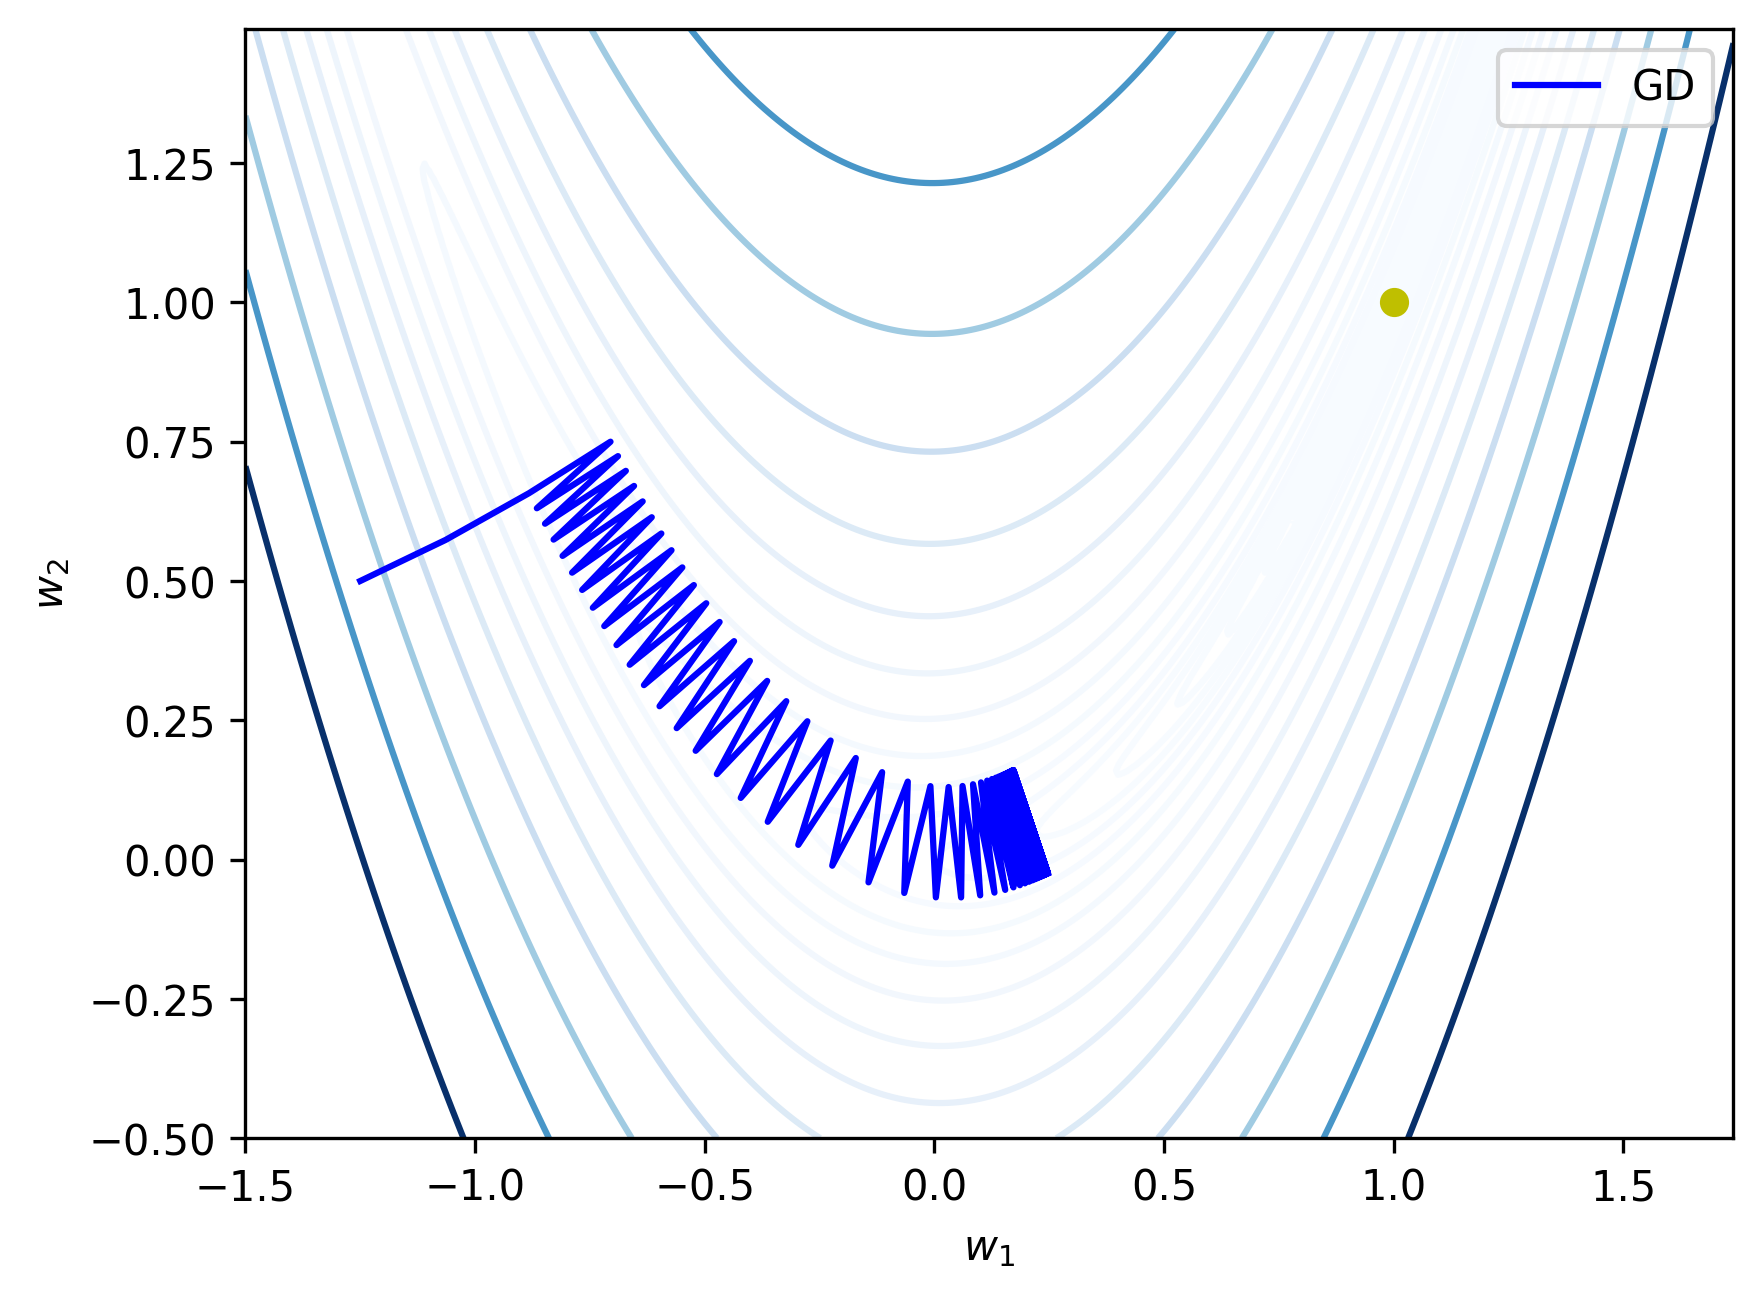
\includegraphics[width=0.6\linewidth]{chapters/neural/images/gd_oscillating.png}
	\caption{Работа градиентного спуска при минимизации функции Розенброка. Метод всегда шагает на фиксированное расстояние чтобы было видно осцилляции.}
	\label{img:gd_osc}
\end{figure}

На решение этих проблем и направлены различные эвристики и обобщения, которые мы рассмотрим далее.

\begin{problem}[Медленная сходимость градиентного спуска.]
Пусть минимизируемая функция имеет следующий вид: $\mathcal{L}(w, x) = (w - w^*)^T M (w - w^*)$, где $M \in \mathbb{R}^{m \times m}$~--- положительно определенная матрица с собственными числами $\lambda_1 = 1$, $\lambda_m = 10^{-4}$. Вычислите величину градиентного шага  $h$, при которой градиентный спуск с постоянным шагом будет гарантированно сходиться. Сколько при такой величине шага потребуется итераций для достижения требуемой точности $\varepsilon$, если точка старта $x_0 = v_m$, где $v_m$~--- собственный вектор матрицы $M$, соответствующий собственному числу $\lambda_m$ и имеющий единичную норму?
\end{problem}

\begin{remark}
Сценарий из этой задачи особенно части встречается, если не отнормировать данные перед обучением модели. 
\end{remark}

\subsection{Метод накопления инерции}

Чтобы избежать осцилляций и сделать стохастический градиентный спуск более плавным, можно добавить градиенту <<инерцию>>, и усреднять его значение по последним нескольким шагам. Тогда получится метод \textbf{Momentum}, или метод тяжелого шарика, изобретенный Б. Т. Поляком в 1964 г. Его метод обновления весов может быть записан так:
\begin{align*}
v &:= \gamma v + (1 - \gamma) \mathcal{L}'(w, x_i) \\
w &:= w - h v\,,
\end{align*}
где параметр $h$ отвечает за величину шага, а $\gamma$~--- за то, насколько сильно предыдущие итерации будет влиять на текущую.

Развил эту идею Ю. Е. Нестеров, в 1983 г. предложив метод \textbf{NAG} (Nesterov's accelerated gradient). В нём градиент не только усредняется по нескольким итерациям, но и <<подглядывает>> вперед в направлении своего движения, и обновляет веса с учетом полученной информации:
\begin{align*}
v &:= \gamma v + (1 - \gamma) \mathcal{L}'(w - h \gamma v, x_i) \\
w &:= w - h v\,,
\end{align*}

Эти методы хорошо показали себя при обучении больших нейросетевых моделей. По сравнению с стохастическим градиентным спуском они обладают большей устойчивостью к выбросам, меньше осциллируют.

\begin{figure}[h]
	\centering
	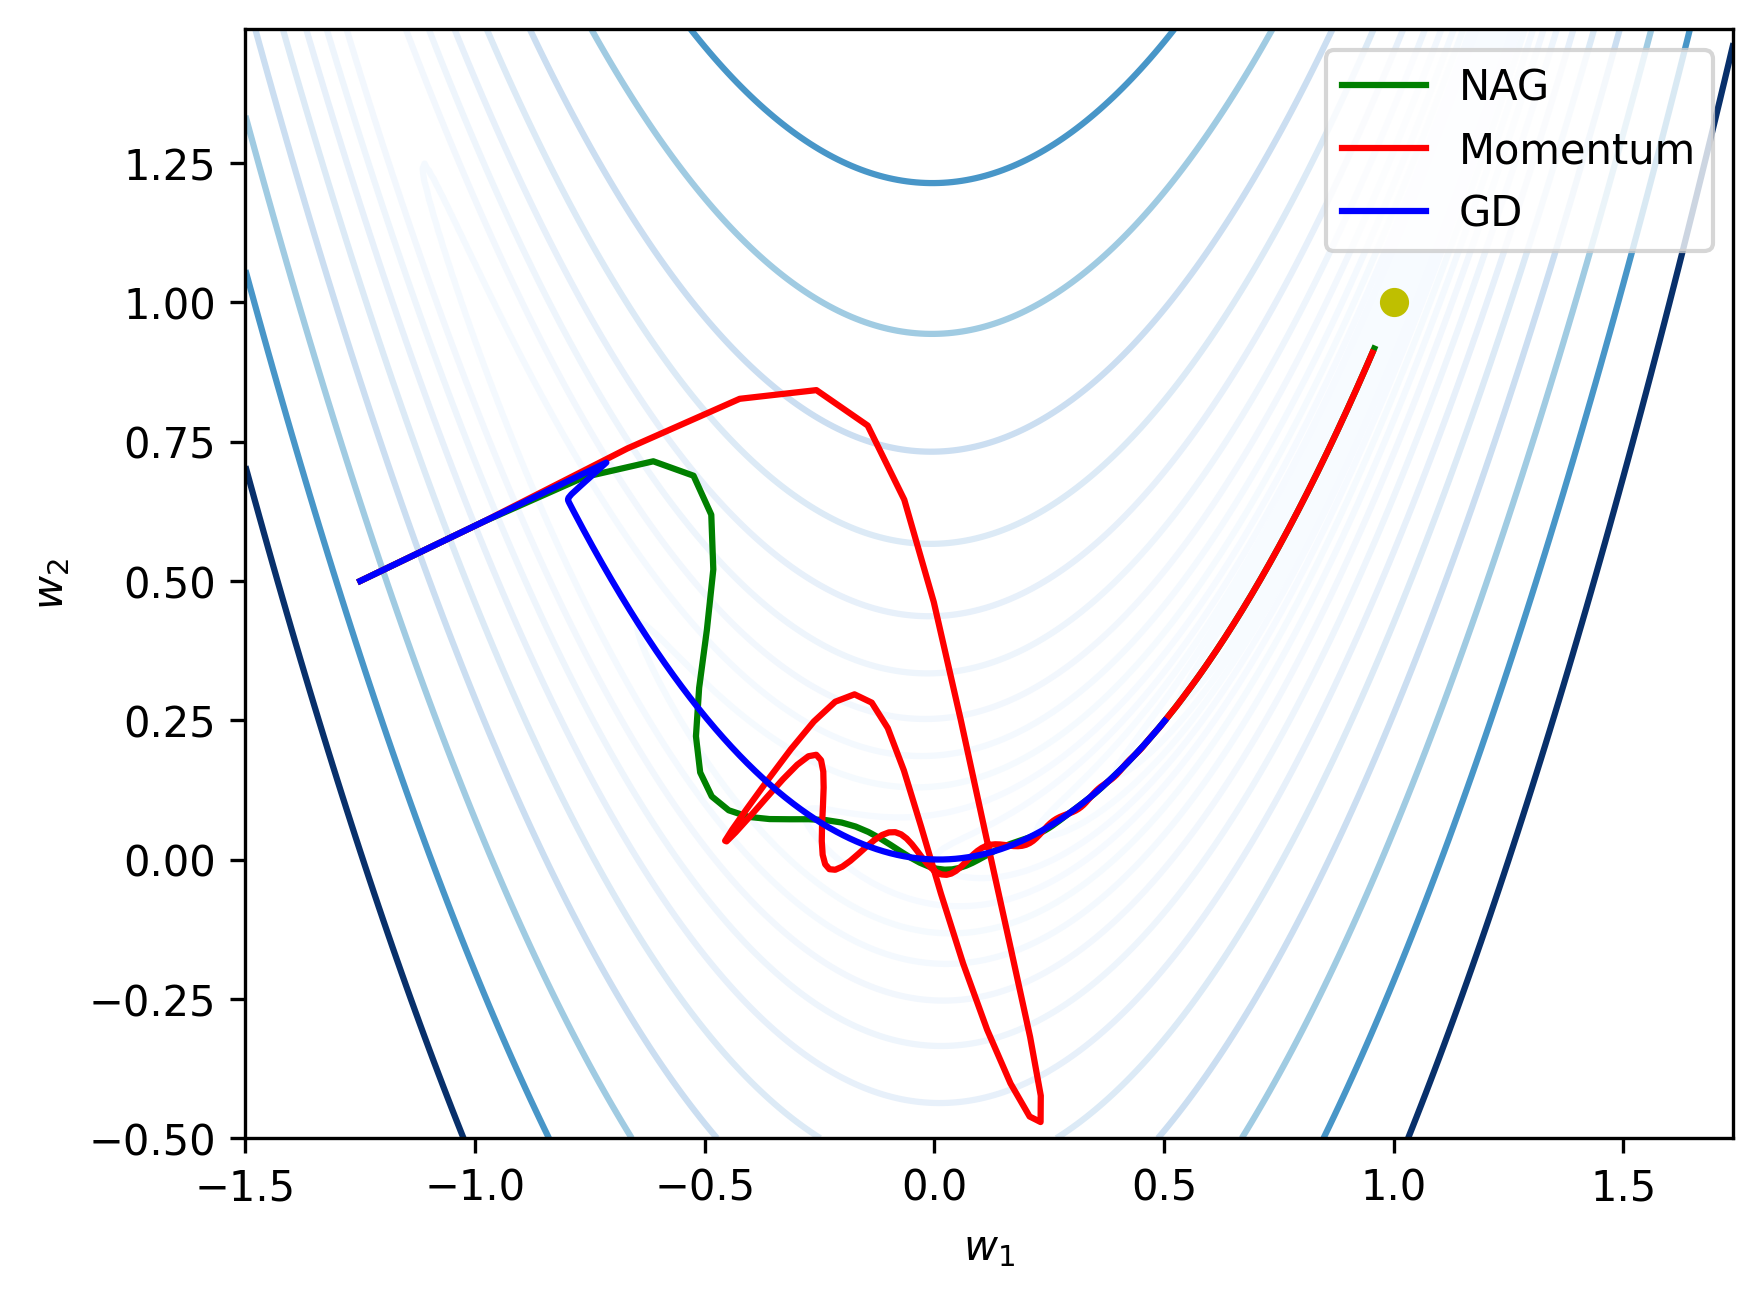
\includegraphics[width=0.6\linewidth]{chapters/neural/images/nag_momentum_gd.png}
	\caption{Пример работы методов Momentum, NAG и градиентного спуска при оптимизации функции Розенброка. Все методы делают $10^4$ итераций.}
	\label{img:gd_osc}
\end{figure}

\subsection{Варианты инициализации весов}

Чтобы улучшить сходимость метода можно правильно инициализировать веса модели. Возможно очень много различных вариантов, например:
\begin{enumerate}
    \item $w_j := 0$ для всех $j=1,\dots,n$;
    \item Небольшие случайные значения, $w_j := \text{random}\left(-\frac{1}{2n}, \frac{1}{2n}\right)$;
    \item Обучение по небольшой стартовой предвыборке объектов;
    \item Мультистарт: многократные запуски из различных случайных начальных приближений и выбор лучшего из них;
    \item В случае линейной регрессии, $w_j := \frac{\langle y, f_j \rangle}{\langle f_j, f_j \rangle}$, где $f_j = (f_j(x_i))_{i=1}^l$.
\end{enumerate}

\begin{problem}[Смысл 5 способа инициализации весов.]
Покажите что в модели линейной регрессии с квадратичной функцией потерь и некореллированными признаками ($\langle f_j, f_k \rangle = 0,\ j \neq k$), веса, полученные с помощью оценки 5 на самом деле являются точным решением задачи оптимизации.
\end{problem}

\subsection{Варианты порядка предъявления объектов}

Метод стохастического градиента чувствителен к тем способу предоставления новых оъектов на каждом шаге. Для улучшения сходимости можно применить одну из следующих эвристик:

\begin{enumerate}
    \item Перетасовка объектов (shuffling). Можно перемешивать объекты, брать попеременно объекты из разнвх классов. Это помогает избежать переобучения если объекты, например, хранятся в хронологическом порядке.
    \item Чаще брать объекты на которых функция потерь принимает большие значения. Это помогает нейросети выучить сложные примеры, даже если в выборке их немного.
\end{enumerate}

В задачах многоклассовой классификации также можно применять следующие техники:
\begin{enumerate}
    \item В задачах классификации чаще брать объекты на которых меньше уверенность (margin).
    \item Вообще не брать <<хорошие>> объекты на которых margin больше константы $\mu_+$. Это может ускорить сходимость.
    \item Вообще не брать объекты <<выбросы>> на которых margin меньше константы $\mu_-$. Это может улучшить качество классификации. 
\end{enumerate}
В этих случаях константы $\mu_+$ и $\mu_-$ придется подбирать.

\subsection{Варианты выбора градиентного шага}

Вообще говоря, сходимость метода стохастического градиента с фиксированным шагом это чудо~--- даже для выпуклых функций метод будет осциллировать в окрестности минимума. Чтобы бороться с проблемой осцилляций можно варьировать величину градиентного шага.

\begin{enumerate}
    \item Можно уменьшать величину шага с каждой итерацией. В таком случае для выпуклых функций сходимость гарантируется если:
    \[
    h_t \rightarrow 0,\, \sum_{t = 1}^{\infty} h_t = \infty,\, \sum_{t=1}^{\infty} h_t^2 < \infty
    \]
    В частности можно положить $h_t = 1 / t$.
    \item Можно на каждом шаге выбирать величину шага, минимизирующую функцию одной переменной:
    \[
    \mathcal{L}(w - h \nabla \mathcal{L}(w, x_i), x_i) \rightarrow \min_h\,.
    \]
    Это называется \textbf{метод скорейшего градиентного спуска}.
    \item Можно делать случайные <<пробные>> шаги, которые помогут <<выбить>> функцию из неглубокого локального минимума.
\end{enumerate}

\begin{figure}[h]
	\centering
	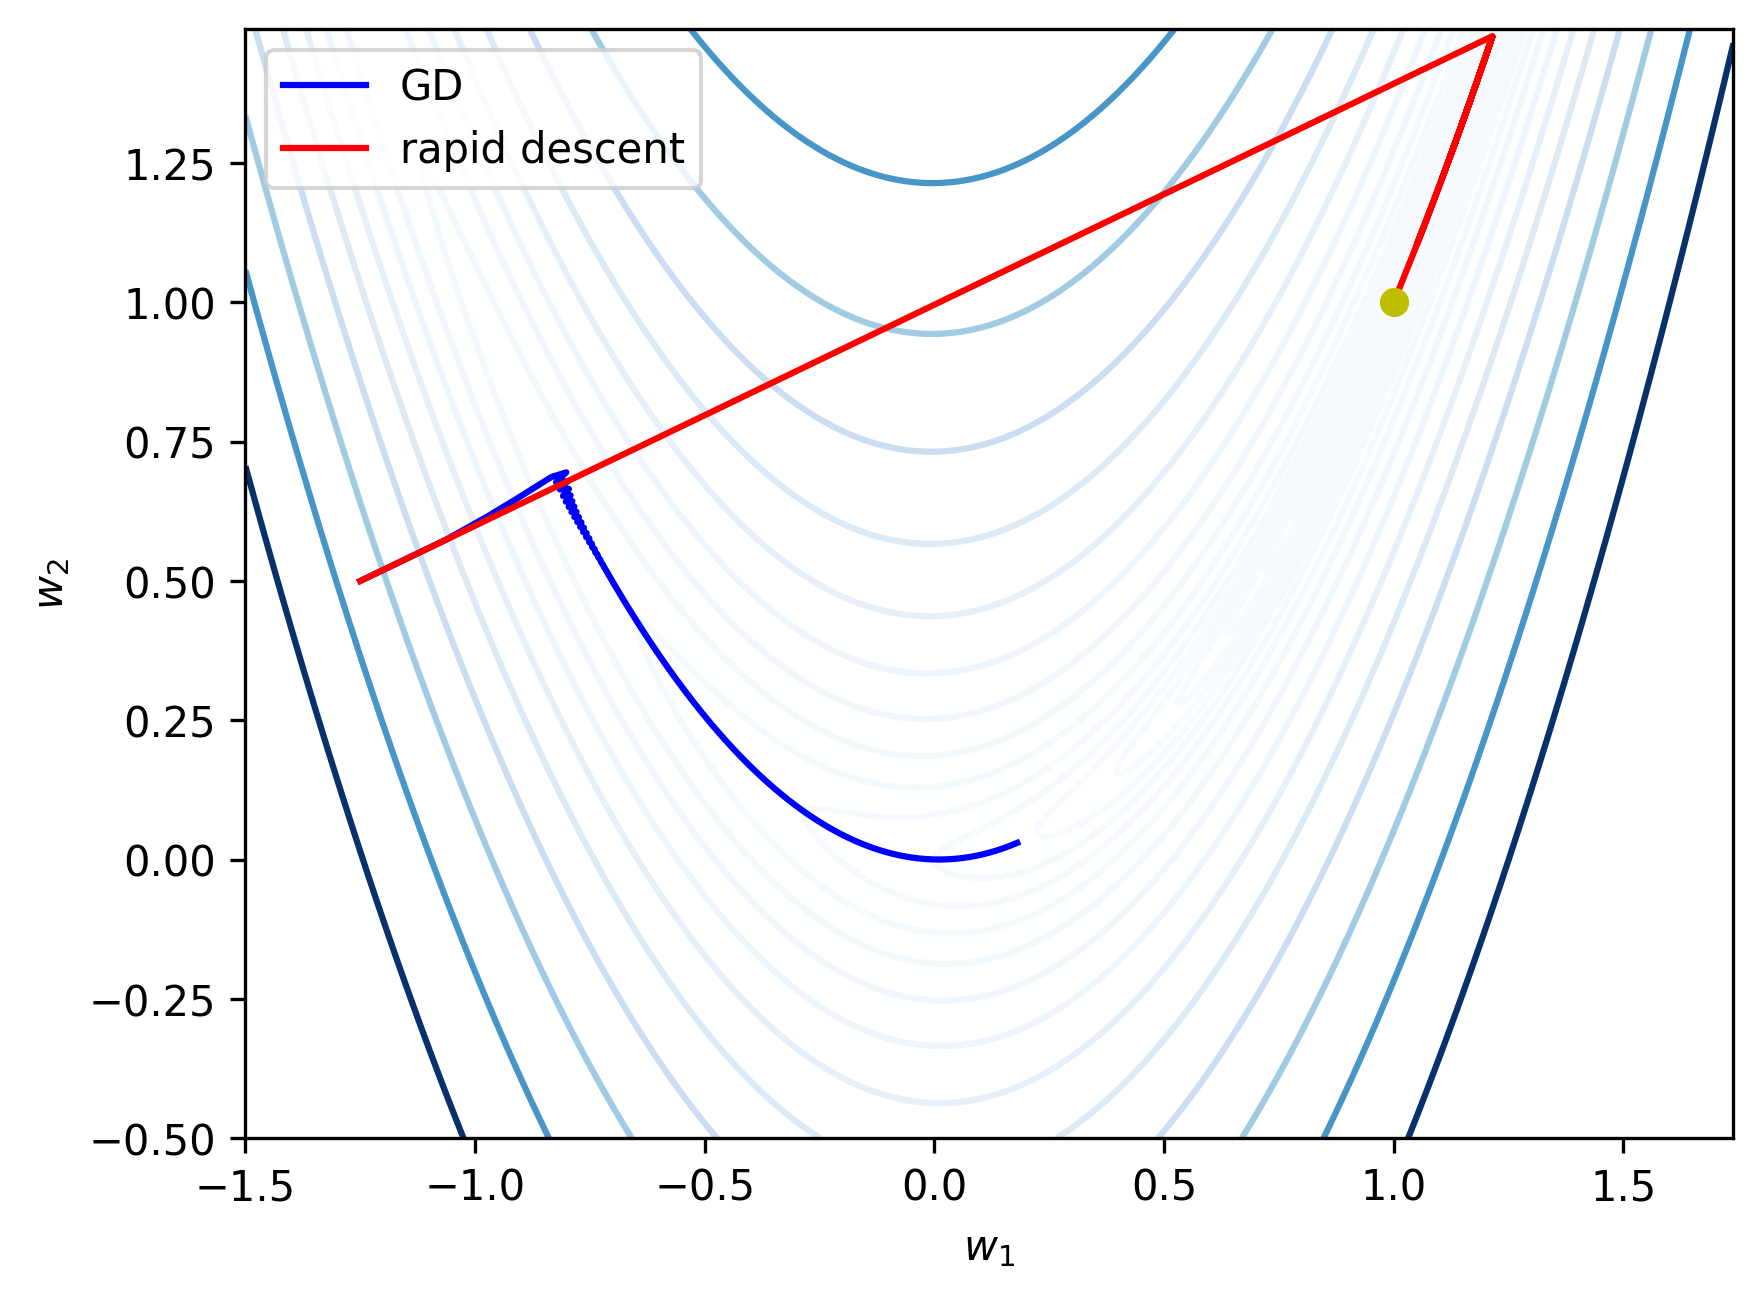
\includegraphics[width=0.6\linewidth]{chapters/neural/images/gd_rd_example.png}
	\caption{Работа градиентного спуска и скорейшего градиентного спуска при минимизации функции Розенброка. Оба метода делают $10^4$ итераций.}
	\label{img:gd_osc}
\end{figure}

\begin{remark}
Существуют и более продвинутые алгоритмы, модифицирующие величину градиентного шага, такие как Adagrad, RMSProp, Adadelta, а также методы, сочетающие идеи подстройки градиентного шага и накопления момента, такие как Adam, Adamax, Nadam. Часть их них будет рассмотрена в последующих параграфах.
\end{remark}

\subsection{Методы второго порядка}

Методы второго порядка используют не только градиент функции, но и ее гессиан. Это может дать очень хорошие результаты, например метод не будет застревать в седловых точках. Методы второго порядка предоставляют более быструю сходимость и точность ценой вычислительной эффективности, и в больших задачах они обычно не применяются.

Самый первый из методов второго порядка~--- многомерный метод Ньютона. Его итерацию можно записать как:
\[
w := w - \left(\nabla^2\mathcal{L}(w, x_i)\right)^{-1}\nabla \mathcal{L}(w, x_i)\,.
\]
Исходно метод Ньютона был предназначен для нахождения нуля функции, и выражение выше представляет собой просто-напросто метод для поиска нулей Гессиана. Однако в такой базовой формулировке метод очень часто расходится, и применятются его различные модификации, такие как метод Ньютона-Рафсона:
\[
w := w - h\left(\nabla^2\mathcal{L}(w, x_i)\right)^{-1}\nabla \mathcal{L}(w, x_i)\,.
\]
где $h$ может быть как постоянной, так и выбираться из соображений минимизации одномерной функции, как в методе скорейшего градиентного спуска.

Есть и огромное количество других обобщений, например метод Левенберга-Маквардта, который представляет собой суперпозицию методов Ньютона-Рафсона и обычного градиентного спуска.

\begin{problem}[Сравнение методов первого и второго порядков]
    Докажите, что если минимизируемая функция квадратична, $\mathcal{L}(w, x) = (w - w^*)^T M (w - w^*)$, где $M$~--- положительно определенная матрица, метод Ньютона сойдется к минимуму за одну итерацию. Сравните вычислительную алгоритма сложность с той, которую вы получили в первой задаче для $\varepsilon = 10^{-8}$
\end{problem}

\section{Функции активации ReLU и PReLU. Проблема «паралича» сети.}
\subsection{Про функции активации}

Функция активации в контексте нейронных сетей определяет выходной сигнал нейрона на основе входного сигнала или набора входных сигналов. Она играет важную роль в определении нелинейности модели и позволяет нейронной сети обучаться сложным зависимостям между входными данными и выходами, а также влияеть на эффективность обучения модели.(грубо говоря определяет будет ли нейрон активирован - даст не нулевой выход) \\
В искусственных нейронных сетях используются различные типы функций активации, такие как тождественная функция, ступенчатые функции, сигмоидные функции и многие другие. \\
\textbf{Важным требованием} к функции активации является ее нелинейность, чтобы нейронная сеть могла эффективно справляться с нетривиальными задачами.\\ Примером широко используемой функции активации является ReLU.

\subsection{ReLU (Rectified Linear Unit), проблема «паралича» сети}

\textbf{\textit{Определение:}} 
Функция активации ReLU определяется как:
$f(x) = max(0, x)$, где x — входное значение.\\
Не смотря на очевидную простоту функции активации ReLU, у неё есть одна существенная проблема: она может вызывать так называемый \textbf{«паралич» сети}.\\
Если градиент весов становится слишком большим, то некоторые нейроны могут получить очень большие отрицательные веса, что приведёт к тому, что их выходные значения всегда будут равны нулю независимо от входного сигнала. Эти нейроны становятся неактивными («замороженными») и больше не участвуют в процессе обучения. Если это происходит слишком часто, то это может привести к ухудшению результата.\\
Для решения этой проблемы была предложена модификация ReLU.
\subsection{PReLU (Parametric Rectified Linear Unit)}

\textbf{\textit{Определение:}}
Функция PReLU является обобщением ReLU и определяется как:
$$ f(x) = \begin{cases}
x & \text{if } x > 0 \\
\alpha x & \text{if } x \leq 0
\end{cases} $$
В отличие от обычной ReLU, где все отрицательные значения обнуляются, PReLU вводит дополнительный параметр $\alpha$, который управляет наклоном линии для отрицательных значений. Этот параметр $\alpha$ может быть обучен вместе с другими параметрами сети, что позволяет избежать полного отключения нейронов. То есть даже отрицательный входной сигнал будет вносить вклад в обучение модели, что уменьшает проблему паралича сети и улучшает получаемый результат.

\subsection{Задачи}
\textbf{Задача 1}

Представьте, что вы получили графики функций активации ReLU и PReLU (с заданным параметром $\alpha$) для различных входных значений.\\
Опишите, как выглядит график функции активации ReLU и как он отличается от графика PReLU. Какова роль параметра $\alpha$ в PReLU?\\
\textbf{Решение}

График функции ReLU выглядит как угол, который начинается от нуля и идет вверх с углом 45 градусов для положительных значений.\\
График функции PReLU (Parametric ReLU) также имеет две части, но для отрицательных значений он не обрезается до нуля. Вместо этого, он наклонен под углом, определяемым параметром $\alpha$. \\
Роль параметра $\alpha$ в PReLU:\\
Параметр $\alpha$ определяет наклон линии для отрицательных значений. Если $\alpha$ велико, то выход будет относительно большим даже для небольших отрицательных входов, что позволяет нейрону сохранять некоторую активность. Если $\alpha$ близко к нулю, то функция будет почти горизонтальной для отрицательных значений, что делает нейрон менее активным в этом диапазоне.\\
\textbf{Задача 2.1}

Рассмотрим простой случай использования функции активации ReLU в одном слое нейронной сети. Пусть входной сигнал равен $-4$, а вес этого нейрона равен $10$. Каково будет значение на выходе этого нейрона после применения функции активации ReLU?\\
\textbf{Решение:}

Выходной сигнал до применения функции активации будет равен произведению входа и веса: $-4 \cdot 10 = -40$. После применения функции активации ReLU получаем: $f(-40) = \max(0, -40) = 0$. Таким образом, этот нейрон станет неактивным ("замороженным"), поскольку его выходной сигнал всегда будет нулевым независимо от изменения входного сигнала.\\
\textbf{Задача 2.2}

Пусть теперь используется функция активации PReLU с параметром $\alpha = 0.01$. Рассчитайте значение на выходе того же нейрона, что и в предыдущей задаче, но уже с использованием PReLU.\\
\textbf{Решение:}

После умножения входа и веса получаем тот же результат: $-4 \cdot 10 = -40$. Теперь применяем функцию активации PReLU:

$$ f(-40) = \begin{cases}
-40 & \text{if } (-40) > 0 \\
0.01 \cdot (-40) & \text{if } (-40) \leq 0
\end{cases} $$

Так как $-40 \leq 0$, мы используем вторую часть определения функции: $f(-40) = 0.01 \cdot (-40) = -0.4$. В этом случае нейрон не становится полностью замороженным, так как его выходной сигнал остается отличным от нуля даже при отрицательном входе.\\
\textbf{Задача 3}

Входной сигнал $x$ распределён равномерно на интервале [-10, 10], а вес $w$ нейрона равен 2, параметр $\alpha = 0.1$.\\
Какова вероятность, что нейрон заморозится при использовании каждой из функций ReLU и PReLU?\\
\textbf{Решение:}\\
Для ReLU:\\
Нейрон «замораживается», если выходной сигнал после применения функции активации всегда равен нулю. То есть, если $wx <= 0$.\\
Поскольку $w = 2$, условие $wx <= 0$ эквивалентно $x <= 0$.\\
Вероятность того, что $x$ окажется меньше или равно нулю, равна вероятности того, что $x$ попадет в интервал -10, 0. \textit{Это составляет половину всего диапазона распределения, поэтому вероятность равна 0.5.}\\
При использовании PReLU нейрон никогда не «замерзнет», потому что даже при отрицательных значениях $x$ выходной сигнал будет отличен от нуля благодаря параметру $\alpha$.
\textit{Таким образом, вероятность того, что нейрон «заморозится», равна 0.}

\section{Drop Out}
\subsection{Теоретические сведения}

\textbf{Drop Out} (метод отключения случайных нейронов) - это метод, который представляет собой эффективный подход к борьбе с переобучением в полносвязных нейронных сетях. 

Переобучение может происходить, когда нейроны в сети начинают "запоминать" шум и особенности обучающего набора, вместо того чтобы извлекать общие закономерности. Во время обучения нейронной сети нейроны взаимодействуют друг с другом, и иногда происходит так, что один нейрон начинает исправлять ошибки другого. Это может привести к ситуации, когда в одном слое нейронов образуются большие веса с разными знаками, что делает модель менее стабильной и затрудняет ее обобщение. В таких случаях, даже если модель демонстрирует высокую точность на обучающих данных, она может оказаться неэффективной на тестовых данных.

Идея Drop Out заключается в том, что при обучении случайные нейроны отключаются (то есть возвращают всегда нулевое значение) и не участвуют в данном шаге обучения. В таком случае большие значения весов разных знаков не всегда участвуют в обучении одновременно, и модель стабилизируется.

Обучение с Dropout можно интерпретировать как обучение одновременно $2^N$ моделей (где $N$ ~--- количество нейронов) с разными архитектурами связей. При обучении выбирается модель, наиболее устойчивая к потере доли нейронов; разные части модели решают одну и ту же задачу вместо того, что бы компенсировать ошибки друг друга.

Недостатком Drop Out является более долгое обучение модели в связи со случайностью процесса обучения.

\subsection{Реализация}
При обучении выбирается параметр $p$ ~--- вероятность отключения. Модель обучается с отключением случайных нейронов. Можно отключать в каждом слое долю $p$ нейронов, вместо независимого отключения, чтобы избежать полного отключения одного слоя.

$$x_i^l = \xi_i^l \sum_{j=1}^{K_{l-1}} w_{ij}^l x_j^{l-1} $$

$l$ ~--- номер текущего слоя, $i$ ~--- номер нейрона в этом слое, $K_l$ ~--- кол-во нейронов в слое $l$, $\xi \sim Be(1-p)$ ~--- случайная величина, отвечающая за отключение.

$\left[\xi_i^l\right] = 1-p$, поэтому на этапе применения вводится нормировка:
$$x_i^l = (1-p) \sum_{j=1}^{K_{l-1}} w_{ij}^l x_j^{l-1} $$

Чаще используется \textbf{Inverted Drop Out} для простоты применения:

$$x_i^l = \frac{\xi_i^l}{1-p} \sum_{j=1}^{K_{l-1}} w_{ij}^l x_j^{l-1} $$
~--- при обучении;

$$x_i^l = \sum_{j=1}^{K_{l-1}} w_{ij}^l x_j^{l-1} $$
~--- при применении.

\subsection{Задачи}
\begin{description}
\item[\textbf{Задача 1}] 
    Какие по порядку величины должны быть ограничения на значения $p$, чтобы избежать отключения одного слоя целиком?
\item[\textbf{Решение:}] если в сети $L$ слоёв размерности $K$, то $p \sim (\frac{c}{L})^{1/K}. $
    Тогда вероятность отключения одного слоя $p^K = \frac{c}{L}; $ вероятность функционирования всех слоёв: $\sim (1-p^K)^L = (1-\frac{c}{L})^L \sim e^{-c}$.
    
    Если взять $c\sim 0.01$ , получим вероятность работы сети $\sim 99\%$.
    
    Если $L=4, K=10,$ то $p \sim 54\%$.

\

\item[\textbf{Задача 2}] 
    Сколько шагов обучения нужно провести, чтобы не осталось нейронов, которые были бы выкинуты на каждом шаге (то есть совсем не обучались)?

\item[\textbf{Решение:}] если в сети $N$ нейронов, то вероятность одному нейрону совсем не обучиться в течение $T$ итераций равна $p^T$. Тогда среднее число необученных нейронов равно $Np^T$. Из условия $Np^T<1$ получаем $T>-\log_{p}N = \frac{\ln N}{\ln \frac{1}{p}}$.



%%%%%%%%%%%%%%%%%%%%%%%%%%%%%%%%%%%%%%%%%%%%%%%%%%%%%%%%%%%%%%%%%%%%%%%%%%%%%%%%%%%%%%%%%%%%%%%%%%%%%%%%%%%%%%%%%%%%%%%%%%%%%%%%%%%%%%%%%%%%%%%%%%%%%%%%%%%%%%%%%%%%%%%%%%%%%%%%%%%%%%%%%%%%%%%%%%%%%%%%%%%%%%%%%%%%%%%%%%%%%%%%%%%
\section{Персептрон и модель Изинга}

Персептрон является одной из базовых моделей машинного обучения и может быть интерпретирован как аналог физических систем, в частности, неоднородной модели Изинга. 
Эти аналогии вдохновили развитие ограниченных машин Больцмана (RBM), которые минимизируют энергетическую функцию, что позволяет создавать более устойчивые модели машинного обучения.  

Пусть имеется решётка, на каждом узле которой $i = 1, \dots, N$ расположена дискретная переменная, принимающая одно из двух состояний: $s_i = +1$ или $s_i = -1$. Эти состояния удобно называть \textit{спинами} (или нейронами в контексте персептрона), где $s_i = +1$ соответствует спину вверх, а $s_i = -1$ — спину вниз. 
Взаимодействие отдельного нейрона с остальными нейронами можно выразить через энергетическую функцию:
\[
E[S] = - \sum_i B_i S_i -\sum_{\langle i j \rangle} J_{ij} S_i S_j,
\]
где:
\begin{itemize}
    \item $S_i \in \{-1, 1\}$ — состояние спина;
    \item $J_{ij}$ — коэффициенты взаимодействия;
    \item $B_i$ — внешнее поле.
\end{itemize}
Если в модели присутствует только первый член, то нейроны не взаимодействуют друг с другом, и модель решается тривиально. Второй член отвечает за взаимодействие между соседними нейронами. Обозначение $\langle i j \rangle$ означает, что сумма берётся по всем парам ближайших соседей в решётке.

В отличие от классической модели Изинга, где взаимодействия между спинами задаются фиксированными параметрами $B$ и $J$, в данном подходе (аналогия с полевой теорией Гинзбурга–Ландау) эти параметры являются обучаемыми. Их значения уточняются в процессе обучения нейронной сети.

В вероятностной интерпретации модель Изинга описывается распределением Гиббса:
\[
P(S) = \frac{1}{Z} e^{-\beta E},
\]
где $Z$ — статистическая сумма:
\[
Z = \sum_{\{S_i\}} e^{-\beta E},
\]
а $\beta$ — это обратная температура 
 + нормировка, $\beta = \frac{1}{k_B T}$. При 
$T\rightarrow0$: сеть ведет себя как дискретная оптимизация (модель Изинга).
При $T \rightarrow \infty$: сеть становится шумной, склонной к случайным состояниям.(См. задача.)

С другой стороны, \textbf{Формула активации для бинарного персептрона:}
\[
y = \mathrm{sign}\left(\sum_{i=1}^n w_i x_i + w_0\right),
\]
где:
\begin{itemize}
    \item $x_i$ — входной сигнал;
    \item $w_i$ — вес связи;
    \item $w_0$ — смещение (bias);
    \item $\mathrm{sign}$ — функция активации, возвращающая $+1$ или $-1$.
\end{itemize}

Здесь веса $w_i$ и сигналы $x_i$ можно рассматривать как аналоги $J_{ij}$ и $S_i$, а функция активации $\mathrm{sign}$ моделирует взаимодействие спинов в системе.

Энергетическая функция $E$ в модели Изинга может быть интерпретирована как функция потерь в персептроне:
\[
E = - \mathbf{w}^\top \mathbf{x},
\]
где $\mathbf{w}$ — вектор весов, а $\mathbf{x}$ — входной вектор.

Минимизация энергии в модели Изинга аналогична обучению персептрона, где цель состоит в подборе весов, минимизирующих ошибку классификации.

\subsection{Функции активации и их физический смысл}

Рассмотрим однослойную нейронную сеть размерности $N - 1$ во внутреннем слое с нейронами $s_i$ и одним выходным нейроном $s_1$. Пусть на вход подаётся вектор размерности $M$. В качестве функции активации на выходном нейроне часто используется гиперболический тангенс:
\[
\mathrm{tanh}(B) = \frac{e^{B} - e^{-B}}{e^{B} + e^{-B}}, \quad -B = w_0 + \sum_i w_i s_i.
\]

Как будет показано далее, его выбор связан не только с асимптотическим поведением и хорошими гладкими свойствами. 

Рассмотрим статистическую сумму невзаимодействующих нейронов, умноженную на единицу:
\[
Z[J] = \left.\sum_{\{s_i\}} e^{-B s_i} e^{J s_i} \right|_{J=0}, \quad s_i \in \{\pm 1\}.
\]
Средняя энергия статистических систем определяется как, оно же мат ожидание нейрона $s$ опрделеяется:
\[
\langle s \rangle = \frac{1}{Z} \frac{\partial}{\partial J} Z = \frac{1}{Z} \sum_{\{s_i\}} e^{-B s_i + J s_i} s_i \bigg|_{J=0} = \tanh(-B).
\]
Таким образом, гиперболический тангенс представляет собой среднюю энергию спиновой системы в модели Изинга и моделирует взаимодействие спинов с одной стороны, и с другой, представляет из себя функцию потерь $\mathcal{L}$  персептрона.

\subsubsection*{Распределение нейронов в сети}

Если состояния нейронов скрытого слоя $i \in [2, N]$ известны, они выражаются через компоненты входного вектора и веса модели:
\[
P(s_i) = \frac{1}{Z_i} \exp\left[ w_{0i} s_i + \sum_{j=1}^M w_{ij} s_i x_j \right].
\]
Тогда вероятностное распределение выходного нейрона $i = 1$ задаётся как:
\[
P(s_1 | s_2, s_3, \dots, s_N) = \frac{1}{Z_1} \exp\left[ s_1 \left( w_{01} + \sum_{i=2}^N w_{i1} s_i \right) \right].
\]

Полное вероятностное распределение выходного нейрона будет иметь вид:
\[
P(s_1) = P(s_1 | s_2, \dots, s_N) \prod_{i=2}^N P(s_i) = \frac{1}{\prod_{i=1}^N Z_i} \exp\left[ \sum_{i=1}^N w_{0i} s_i + \sum_{i,j=2}^{N,M} w_{ij} s_i x_j + s_1 \sum_{j=1}^M w_{ij} s_j \right].
\]

Запишем это в терминах модели Изинга:
\[
P(s_1) = \frac{1}{Z} \exp\left[-\sum_i B_i s_i - \sum_{i,j} J_{ij} s_i s_j \right],
\]
где $B_i$ — магнитное поле, а $J_{ij}$ — взаимодействие нейронов, которые выражаются через веса. В процессе обучения модели (backpropagation) задача состоит в определении значений $B_i$ и $J_{ij}$.
Нахождение распределения вероятностей в сети соответствует решению задачи минимизации энергии модели Изинга.

\subsection{Задачи}
\textbf{Задача 1:} Покажите, что вероятностная интерпретация модели Изинга связана с логистической регрессией.

\textbf{Решение:}
Логистическая регрессия основана на функции активации:
\[
\sigma(x) = P(y=1 | x) = \frac{1}{1 + e^{-E}}, \quad E = \mathbf{w}^\top \mathbf{x} + w_0.
\]

Для модели Изинга распределение вероятностей:
\[
P(S = 1) = \frac{e^{-E}}{e^{E} + e^{-E}} = \frac{1}{1+ e^{2E}} =  \sigma(-2E),\quad P(S = -1) = \sigma(2E).
\]
что аналогично модели логистической регрессии с сигмоидальной функцией вероятности.
\textbf{Задачи 2 - 3:}  
Модель весов \( W \) персептрона имеет специальную структуру:
\[
W = \text{Diag}(d_1, d_2, \dots, d_N) + \mathbf{x} \mathbf{x}^\top,
\]
где \( \text{Diag}(d_1, d_2, \dots, d_N) \) — диагональная матрица, а \( \mathbf{x} \mathbf{x}^\top \) — внешнее произведение входного вектора \( \mathbf{x} \). Энергия системы(она же функция потерь) определяется как:
\[
E = -\mathbf{s}^\top W \mathbf{s},
\]
где \( \mathbf{s} \in \{-1, +1\}^N \).

\begin{enumerate}
    \item Найти состояние \( \mathbf{s} \), минимизирующее энергию \( E \).
    \item Найдите общее условие на W, при котором система имеет как минимум два устойчивых состояния $s_1$ и $s_2$. 
\end{enumerate}

\textbf{Решение:}

1. \textbf{Минимум функции энергии:}

Энергия \( E \) принимает вид:
\[
E = -\mathbf{s}^\top \text{Diag}(d_1, \dots, d_N) \mathbf{s} - \mathbf{s}^\top (\mathbf{x} \mathbf{x}^\top) \mathbf{s}.
\]

Первый член:
\[
-\mathbf{s}^\top \text{Diag}(d_1, \dots, d_N) \mathbf{s} = -\sum_{i=1}^N d_i s_i^2.
\]
Так как \( s_i^2 = 1 \) для \( s_i \in \{-1, +1\} \), получаем:
\[
-\mathbf{s}^\top \text{Diag}(d_1, \dots, d_N) \mathbf{s} = -\sum_{i=1}^N d_i.
\]

Второй член:
\[
-\mathbf{s}^\top (\mathbf{x} \mathbf{x}^\top) \mathbf{s} = -(\mathbf{x}^\top \mathbf{s})^2.
\]

Таким образом, энергия принимает вид:
\[
E = -\sum_{i=1}^N d_i - (\mathbf{x}^\top \mathbf{s})^2.
\]

Энергия минимизируется, когда \( (\mathbf{x}^\top \mathbf{s})^2 \) максимально. Это достигается, если компоненты вектора \( \mathbf{s} \) сонаправлены с компонентами \( \mathbf{x} \). То есть:
\[
s_i = \text{sign}(x_i), \quad i = 1, \dots, N.
\]

2. \textbf{Устойчивые состояния:}

Поскольку \( W \) симметрична, энергия может быть минимизирована, если состояния \( \mathbf{s} \) совпадают с собственными векторами матрицы \( W \), соответствующими наименьшим собственным значениям.

\begin{itemize}
    \item Один собственный вектор — это \( \mathbf{x} \) с собственным значением \( \|\mathbf{x}\|^2  + \overline{d}\) (d - взвешенного диагонального элемента по направлению x),
    \item Остальные \( N-1 \) собственных значений равны диагональным элементам \( d_i \).
\end{itemize}

Если \( \|\mathbf{x}\|^2 \gg d_i \), то устойчивое состояние \( \mathbf{s} \) сонаправлено с \( \mathbf{x} \). Если \( d_i \) доминируют, состояние определяется диагональными элементами.

Кроме того, симметрия матрицы \( W \) означает, что если \( \mathbf{s}^* \) минимизирует энергию, то \( -\mathbf{s}^* \) тоже является решением, так как:
\[
E(-\mathbf{s}^*) = E(\mathbf{s}^*).
\]

\textbf{Задача*} 

1. Рассмотрим однослойную нейронную сеть с \( N \) нейронами в скрытом слое и одним выходным нейроном. На вход поступает вектор \( \mathbf{x} \in \mathbb{R}^M \), веса имеют случайные значения \( w_i \sim \mathcal{N}(0, \sigma^2) \), а функция активации на выходном нейроне задается как:
   \[
   s_\text{out} = f\left( \sum_{i=1}^N w_i \cdot s_i + w_0 \right),
   \]
   где \( f(x) = \mathrm{tanh}(\beta x), \beta = 1/T \).

Что произойдет с выходом \( s_\text{out} \) при \( T \to \infty \) и \( T \to 0 \), если считать, что активация тангенса моделирует энергетическое состояние спиновой системы? 

2. Рассмотрим предельный случай, когда число нейронов \( N \to \infty \), а веса \( w_i \) независимы и одинаково распределены. Покажите, что результатирующее распределение выхода \( s_\text{out} \) будет стремиться к гауссовскому. В каком случае это приближение применимо?

\textbf{Решение:}

\subsubsection*{1. Поведение нейронной сети при \( T \to \infty \) и \( T \to 0 \)}

\textbf{При \( T \to \infty \):}
Гиперболический тангенс \( \mathrm{tanh}(\beta x) \) стремится к линейной функции:
\[
\mathrm{tanh}(\beta x) \approx \beta x \quad \text{при } \beta \to 0 \, (T \to \infty).
\]
Нейронная сеть теряет нелинейность, и выход становится линейной комбинацией входов:
\[
s_\text{out} \approx \beta \left( \sum_{i=1}^N w_i s_i + w_0 \right).
\]
Поведение сети приближается к \textbf{линейной модели}.

\textbf{При \( T \to 0 \):}

Гиперболический тангенс становится почти пороговой функцией:
\[
\mathrm{tanh}(\beta x) \to 
\begin{cases} 
-1, & x < 0, \\ 
1, & x > 0.
\end{cases}
\]
Нейронная сеть превращается в \textbf{дискретную систему}, где выходные значения строго определяются знаком линейной комбинации входов:
\[
s_\text{out} = \text{sign} \left( \sum_{i=1}^N w_i s_i + w_0 \right).
\]

\subsubsection*{2. Гауссовское распределение при \( N \to \infty \)}

\textbf{При} \( N \to \infty \), веса \( w_i \) независимы и одинаково распределены (\( w_i \sim \mathcal{N}(0, \sigma^2) \)), а входы \( s_i \in \{-1, 1\} \).
Сумма выходов на входном слое:
\[
S = \sum_{i=1}^N w_i s_i.
\]
По центральной предельной теореме:
\begin{itemize}
    \item Среднее \( \mu = \mathbb{E}[S] = 0 \) (поскольку \( \mathbb{E}[w_i] = 0 \) и \( \mathbb{E}[s_i] = 0 \)).
    \item Дисперсия \( \sigma^2 = N \cdot \mathbb{V}[w_i] \cdot \mathbb{V}[s_i] = N \sigma^2 \).
\end{itemize}
При \( N \to \infty \), \( S \) стремится к распределению:
\[
S \sim \mathcal{N}(0, N \sigma^2).
\]
Это верно при конечном $T$, Активация 
$\tanh$ сжимает значение $z \in [-1, 1]$, поскольку функция гладкая, форма распределения не меняется и зависит от двух моментов.
%%%%%%%%%%%%%%%%%%%%%%%%%%%%%%%%%%%%%%%%%%%%%%%%%%%%%%%%%%%%%%%%%%%%%%%%%%%%%%%%%%%%%%%%%%%%%%%%%%%%%%%%%%%%%%%%%%%%%%%%%%%%%%%%%%%%%%%%%%%%%%%%%%%%%%%%%%%%%%%%%%%%%%%%%%%%%%%%%%%%%%%%%%%%%%%%%%%%%%%%%%%%%%%%%%%%%%%%%%%%%%%%%%%


\section{CNN. Свёртки и пулинги для обработки изображений.}
\subsection{Стандартная схема свёрточной сети.}

$ x[i, j] $ — исходные признаки, пиксели $ n \times m $-изображения

$ w_{ab} $ — ядро свёртки, $ a = -A, \ldots, +A $, $ b = -B, \ldots, +B $

Неполносвязный свёрточный нейрон с $ (2A + 1)(2B + 1) $ весами:

$$
(x * w)[i, j] = \sum_{a=-A}^{A} \sum_{b=-B}^{B} w_{ab} \, x[i + a, j + b]
$$

Объединяющий нейрон — это необучаемая свёртка с шагом $ h > 1 $, агрегирующая данные прямоугольной области $ h \times h $(объединяющий слой нейронов = пулинг слой):

$$
y[i, j] = F \left( x[hi, hj], \ldots, x[hi + h - 1, hj + h - 1] \right)
$$

где  F  — агрегирующая функция: max, average и т.п. Max-pooling позволяет обнаружить элемент в любой из ячеек.

\begin{figure}[h]

\centering

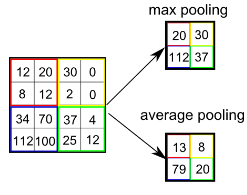
\includegraphics[width=0.2\linewidth]{chapters/neural/images/пуллинг.png}

\label{fig:pulling}

\end{figure}

\begin{figure}[h]

\centering

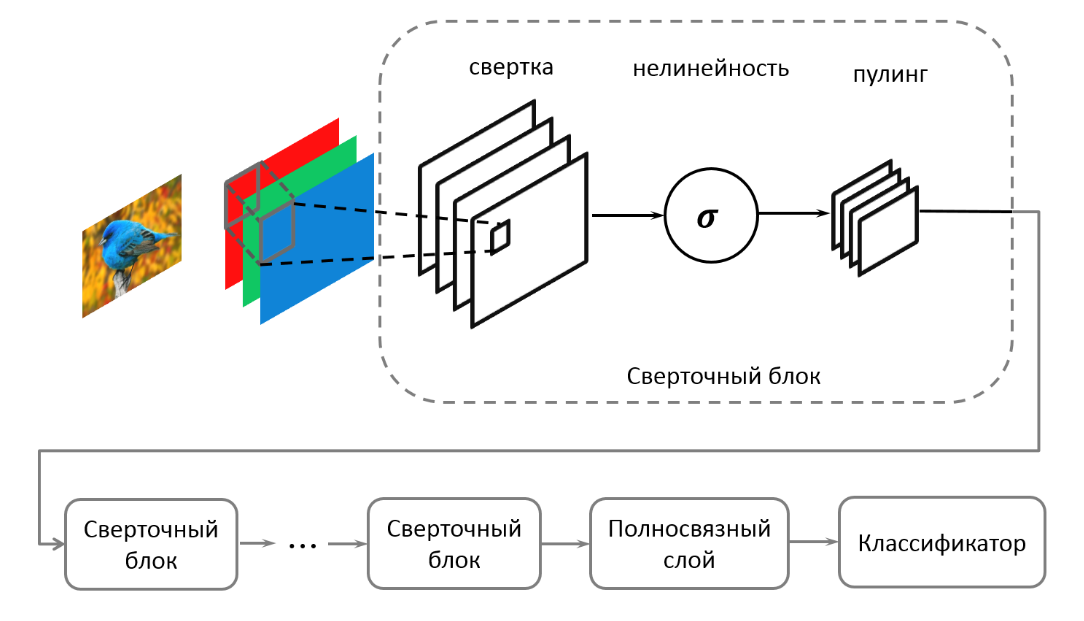
\includegraphics[width=0.8\linewidth]{chapters/neural/images/1CNN.png}

\label{fig:one_cnn}

\end{figure}

Свёрточная сеть обучается извлечению признаков

Чем выше слой, тем более крупные и сложные элементы изображений он способен распознавать

\newpage
\subsection{Приложения CNN.}

Классификация изображений( Свёрточная сеть \textbf{AlexNet} )\\

Распознавание речевых сигналов\\
\begin{figure}[h]

\centering

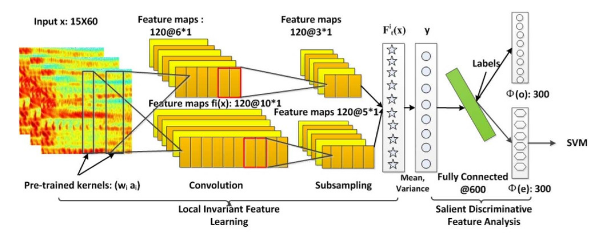
\includegraphics[width=0.8\linewidth]{chapters/neural/images/pic.png}

\label{fig:voice_signals_nn}

\end{figure}

Классификация предложений в тексте:\\
Последовательные слова в тексте представляются векторами с помощью векторных представлений (word2vec и др.)\\

\newpage
\subsection{Обобщение CNN на любые структурированные данные.}
Допустим, каждый объект имеет структуру, заданную графом

\textbf{Свёртка} определяется по локальной окрестности вершины

\textbf{Пулинг} агрегирует векторы вершин локальной окрестности

Такая сеть обучается находить и классифицировать подграфы

\begin{figure}[h]

\centering

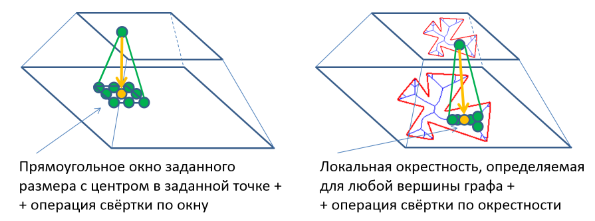
\includegraphics[width=0.8\linewidth]{chapters/neural/images/обобщениеCNN.png}

\label{fig:cnn_generalization}

\end{figure}

\subsection{Задачи}
\textbf{Задача 1}

Дано изображение размером 5x5 пикселей и свёрточное ядро размером 3x3 пикселя\\

\begin{equation*}
\begin{Vmatrix}
1 & 2 & 3 & 0 & 1\\
4 & 5 & 6 & 1 & 0\\
7 & 8 & 9 & 2 & 1\\
0 & 1 & 2 & 3 & 4\\
1 & 0 & 1 & 0 & 1
\end{Vmatrix}
""
\begin{Vmatrix}
1 & 0 & -1\\
1 & 0 & -1\\
1 & 0 & -1
\end{Vmatrix}
\end{equation*}
Необходимо выполнить операцию свёртки\\
\textbf{Решение}

1.Результирующая матрица после свёртки будет размером
$$ (5-3+1) \times (5-3+1) = 3 \times 3 $$.

2. Процесс свёртки:

Для каждого положения свёрточного ядра на изображении вычисляем\\
сумму произведений.

Позиция (0,0):
$
(1 \times 1) + (2 \times 0) + (3 \times -1) + \\
(4 \times 1) + (5 \times 0) + (6 \times -1) + \\
(7 \times 1) + (8 \times 0) + (9 \times -1) = \\
1 + 0 - 3 + 4 + 0 - 6 + 7 + 0 - 9 = -6
$

 Позиция (0,1):
$
(2 \times 1) + (3 \times 0) + (0 \times -1) + \\
(5 \times 1) + (6 \times 0) + (1 \times -1) + \\
(8 \times 1) + (9 \times 0) + (2 \times -1) = \\
2 + 0 + 0 + 5 + 0 - 1 + 8 + 0 - 2 = 12
$

Позиция (0,2):
$
(3 \times 1) + (0 \times 0) + (1 \times -1) + \\
(6 \times 1) + (1 \times 0) + (2 \times -1) + \\
(9 \times 1) + (2 \times 0) + (1 \times -1) = \\
3 + 0 - 1 + 6 + 0 - 2 + 9 + 0 - 1 = 16
$

Позиция (1,0):
$
(4 \times 1) + (5 \times 0) + (6 \times -1) + \\
(7 \times 1) + (8 \times 0) + (9 \times -1) + \\
(0 \times 1) + (1 \times 0) + (2 \times -1) = \\
4 + 0 - 6 + 7 + 0 - 9 + 0 + 0 - 2 = -6
$

Позиция (1,1):
$
(5 \times 1) + (6 \times 0) + (1 \times -1) + \\
(8 \times 1) + (9 \times 0) + (2 \times -1) + \\
(1 \times 1) + (0 \times 0) + (3 \times -1) = \\
5 + 0 - 1 + 8 + 0 - 2 + 1 + 0 - 3 = 8
$

Позиция (1,2):
$
(6 \times 1) + (1 \times 0) + (0 \times -1) + \\
(9 \times 1) + (2 \times 0) + (1 \times -1) + \\
(2 \times 1) + (3 \times 0) + (4 \times -1) = \\
6 + 0 + 0 + 9 + 0 - 1 + 2 + 0 - 4 = 12
$

Позиция (2,0):
$
(7 \times 1) + (8 \times 0) + (9 \times -1) + \\
(0 \times 1) + (1 \times 0) + (2 \times -1) + \\
(1 \times 1) + (0 \times 0) + (3 \times -1) = \\
7 + 0 - 9 + 0 + 0 - 2 + 1 + 0 - 3 = -4
$

Позиция (2,1):
$
(8 \times 1) + (9 \times 0) + (2 \times -1) + \\
(1 \times 1) + (2 \times 0) + (3 \times -1) + \\
(0 \times 1) + (1 \times 0) + (4 \times -1) = \\
8 + 0 - 2 + 1 + 0 - 3 + 0 + 0 - 4 = 0
$

Позиция (2,2):
$
(9 \times 1) + (2 \times 0) + (1 \times -1) + \\
(2 \times 1) + (3 \times 0) + (4 \times -1) + \\
(1 \times 1) + (0 \times 0) + (1 \times -1) = \\
9 + 0 - 1 + 2 + 0 - 4 + 1 + 0 - 1 = 6
$

После выполнения всех операций свёртки\\
мы получаем следующую матрицу:

$$
\begin{Vmatrix}
-6 & 12 & 16 \\
-6 & 8 & 12 \\
-4 & 0 & 6 \\
\end{Vmatrix}
$$

\newpage
\textbf{Задача 2}

Даны изображения продукции с производственной линии.\\
К сожалению, некоторые с дефектами.\\
Предоставьте алгоритм построения CNN для распознавания дефектов на изображениях.

\textbf{Подойдёт такое решение:}

\begin{enumerate}
    \item Создать CNN с тремя свёрточными слоями и двумя pooling-слоями.
    \item Использовать dropout для предотвращения переобучения.
    \item Добавить полносвязный слой перед выходным слоем.
    \item Взять сигмоидный выходной слой для бинарной классификации.
    \item Обучить модель на размеченных изображениях, используя функцию потерь бинарная кросс-энтропия.\end{enumerate}\\

\textbf{Задача 3}

Каковы основные компоненты CNN и их функции?\\
\textbf{Решение:}
\begin{itemize}
    \item Свёрточные слои: применяют свёртку к входным данным, чтобы выделить важные признаки.
    \item Слои подвыборки(Pooling): уменьшают размерность данных, сохраняя наиболее значимую информацию.
    \item Полносвязные слои: используются для окончательной классификации на основе извлечённых признаков.
\end{itemize}

\end{description}


\section*{Оптимальное прореживание нейронных сетей}

\subsection*{Введение}
Прореживание нейронных сетей (англ. optimal brain damage) — метод упрощения структуры регрессионной модели, например, нейронной сети. Основная идея прореживания (англ. pruning) заключается в том, что те элементы модели или те нейроны сети, которые оказывают малое влияние на ошибку аппроксимации, можно исключить из модели без значительного ухудшения качества аппроксимации \cite[VorontsovOptBrainDamage].
Такой подход позволяет достичь следующих целей:
\begin{itemize}
    \item \textbf{Сжатие нейросети.} Уменьшается количество параметров, которые нужно хранить, что важно для устройств с ограниченными ресурсами.
    \item \textbf{Ускорение вычислений.} Меньшее количество параметров требует меньше операций умножения, что ускоряет работу модели.
    \item \textbf{Регуляризация.} Снижение числа параметров уменьшает склонность модели к переобучению, делая её более устойчивой к шуму данных.
    \item \textbf{Повышение качества.} Часто итоговая модель после прореживания показывает лучшие результаты, чем исходная.
    Это связано с тем, что избыточно сложная модель склонна к переобучению, а последовательное исключение избыточных параметров позволяет оптимально адаптировать её сложность к задаче.
\end{itemize}

\subsection*{История метода}
Метод второго порядка был предложен Яном ЛеКуном в 1990 году \cite{lecun1990optimal} и получил название \textit{Optimal Brain Damage}.
На тот момент этот подход был одним из лучших для уменьшения размеров нейронных сетей и улучшения их качества.
Позднее Хассиби и Штурм \cite{hassibi1993optimal} разработали его улучшение \textit{Optimal Brain Surgery}, основываясь на анализе вторых производных. 
Ранее существовали методы нулевого порядка, где исключались элементы с малыми весами \cite{mozer1989skeletonization}.
В 1990 году А. Н. Горбань предложил метод, использующий первые производные, что позволило обойтись без вычисления вторых производных. 
Этот подход получил название \textit{контрастирование нейронных сетей}. Е. М. Миркес развил идеи Горбаня, создав библиотеку функций и язык описания для проекта «Идеального нейрокомпьютера».

Впоследствии появились более современные методы, например Dropout, $L_2$-регуляризация и другие, которые вытеснили этот подход из основного арсенала.
Тем не менее, метод прореживания всё ещё может быть полезным инструментом, особенно в ситуациях, требующих компактности модели.

\subsection*{Математическая постановка задачи}
Рассмотрим регрессионную модель 
\[
y_n = f(\mathbf{w}, \mathbf{x}_n) + \nu,
\]
где $\mathbf{w} \in \mathbb{R}^d$ — вектор параметров, $\mathbf{x}_n \in \mathbb{R}^p$ — вектор независимых переменных, $y_n \in \mathbb{R}$ — зависимая переменная, $\nu$ — случайная ошибка. 

Задана выборка $D = \{(\mathbf{x}_n, y_n)\}_{n=1}^N$. Для минимизации функции ошибки 
\[
E_D(\mathbf{w}) = \sum_{n=1}^N \ell(y_n, f(\mathbf{w}, \mathbf{x}_n)),
\]
где $\ell(\cdot, \cdot)$ — функция потерь, требуется найти $\mathbf{w}^{MP} = \arg\min_{\mathbf{w}} E_D(\mathbf{w})$. 

\subsection*{Прореживание параметров}
Цель метода — исключение параметров $w_i$, которые оказывают наименьшее влияние на ошибку $E_D$.
Для этого используется квадратичная аппроксимация $E_D$ в окрестности $\mathbf{w}^{MP}$:
\[
E_D(\mathbf{w} + \Delta\mathbf{w}) \approx E_D(\mathbf{w}^{MP}) + \frac{1}{2} \Delta\mathbf{w}^T H \Delta\mathbf{w},
\]
где $H = \nabla^2_{\mathbf{w}} E_D(\mathbf{w}^{MP})$ — матрица Гессе.

Исключение параметра $w_i$ эквивалентно наложению ограничения $\Delta w_i + w_i = 0$.
Для выполнения данного условия минимизируется функция:
\[
\Delta E_D = \frac{1}{2} \Delta\mathbf{w}^T H \Delta\mathbf{w},
\]
при ограничении $\mathbf{e}_i^T \Delta\mathbf{w} + w_i = 0$, где $\mathbf{e}_i$ — единичный вектор с $i$-м элементом, равным $1$. 

\subsection*{Оптимизация}
Используем метод множителей Лагранжа для минимизации:
\[
S = \frac{1}{2} \Delta\mathbf{w}^T H \Delta\mathbf{w} - \lambda (\mathbf{e}_i^T \Delta\mathbf{w} + w_i).
\]
Дифференцируя $S$ по $\Delta\mathbf{w}$ и $\lambda$ и приравнивая производные к нулю, получаем:
\[
\Delta\mathbf{w} = -\frac{w_i}{[H^{-1}]_{ii}} H^{-1} \mathbf{e}_i.
\]
Подставляя это выражение в $\Delta E_D$, находим:
\[
L_i = \frac{w_i^2}{2 [H^{-1}]_{ii}}.
\]
Параметр $i$, минимизирующий $L_i$, выбирается для исключения.

\subsection*{Итеративный процесс прореживания}
Вышенаписанный процесс можно повторять несколько раз для повышения эффиктивности модели:
\begin{enumerate}
    \item Определяется вес, который оказывает минимальное влияние на ошибку, и он исключается из модели.
    Удаление выполняется до тех пор, пока ошибка не превышает заданный порог.
    \item После удаления части параметров модель дообучается, чтобы восстановить её качество.
    \item Процесс повторяется, пока не будет достигнута желаемая компактность или качество модели или пока не пройдет заданное число итераций.
\end{enumerate}

\subsection*{Задачи}
\begin{task}
Выпишите Лагранжиан для решения задачи нахождения веса, зануление которого ведет к минимальной ошибке для методов 3 и 4 порядков. Попробуйте решить эту оптимизационную задачу.
\end{task}

\begin{task}
Мы раскладываем функции ошибки до второй производной, хотя приращение $\Delta w_i = -w_i$ может быть достаточно большим. Оцените применимость данного метода в зависимости от величины весов $w_i$.
\end{task}

\begin{task}
Рассчитайте $L_i$ для модели, в которой $H = \begin{bmatrix} 4 & 2 \\ 2 & 3 \end{bmatrix}$, $w = \begin{bmatrix} 1 \\ -2 \end{bmatrix}$.
\end{task}

\section{Batch normalization}

\subsection{Введение}
В основе Batch Normalization лежит решение проблемы «внутреннего ковариационного сдвига» (Internal Covariate Shift). Этот термин описывает явление, при котором распределение входных данных каждого слоя нейронной сети меняется в процессе обучения, из-за чего сети становится сложнее обучать. Это происходит из-за того, что параметры предыдущих слоев изменяются во время обучения, влияя на данные текущего слоя.

Batch Normalization решает эту проблему, нормализуя выход каждого слоя. Нормализация заключается в преобразовании входных данных каждого слоя таким образом, чтобы среднее значение было приближено к нулю, а стандартное отклонение — к единице. Это делает сеть менее чувствительной к масштабу входных данных и улучшает общую стабильность процесса обучения.

Причина популярности batch normalization заключается в значительном ускорении обучения нейронных сетей и в улучшении их сходимости в целом. Его использование гарантирует, что каждая компонента представления на выходе будет иметь контролируемое среднее и дисперсию.

\subsection{Алгоритм}
Сперва идёт слой batch normalization, на котором текущий батч приводится к нулевому среднему и единичной дисперсии, где $\mu$ и $\sigma^2$ - среднее и дисперсия признаков по обрабатываемому батчу, $\varepsilon$ - гиперпараметр слоя, служащий для численной устойчивости.

\[X^{k+1} = \frac{X^k - \mu}{\sqrt{\sigma^2 + \varepsilon}}\]

Далее идёт слой channelwise scaling, который позволяет выучить оптимальное шкалирование для всех признаков $X^{k+2}$. Где $beta$ и $\gamma$ - обучаемые параметры, позволяющие настраивать в ходе обучения оптимальные значения матожидания и дисперсии выходного слоя.

\[X^{k+2} = \beta X^{k+1} + \gamma \]

В ходе предсказания мы используем $\mu_*$ $\sigma_*^2$, полученные в ходе обучения как скользящее среднее всех средних и дисперсий. 

\subsection{Задачи}

\subsubsection*{Задача 1}
Рассмотрим ситуацию: у вас есть небольшой набор данных, и мини-батчи содержат только по 2-3 образца. Какие проблемы могут возникнуть при использовании Batch Normalization в таких условиях? Какие методы можно использовать для решения этих проблем?

\subsubsection*{Задача 2}
Как параметры скользящих статистик влияют на работу модели?

\subsubsection*{Задача 3}
Почему нельзя использовать статистики конкретного батча во время предсказания


\section{Методы оптимизации с использованием Autograd: SGD, Adam, RMSProp}

\subsection{Автоматическое дифференцирование с Autograd}

Autograd \textendash{} это инструмент для автоматического дифференцирования, который позволяет автоматически вычислять градиенты функций. В контексте методов оптимизации, Autograd упрощает процесс нахождения производных для сложных функций потерь. Благодаря Autograd, пользователю не нужно вручную выводить градиенты \textendash{} они вычисляются программно с использованием обратного распространения (backpropagation).

Autograd используется во многих популярных библиотеках, таких как \texttt{PyTorch} и \texttt{JAX}. На семинарах были продемонстрированы примеры использования Autograd для автоматического вычисления градиентов при оптимизации нейронных сетей.

\subsubsection{Пример использования Autograd}

Предположим, у нас есть функция потерь $L(\theta) = (\theta^2 + 3\theta + 2)$. С помощью Autograd можно вычислить градиент этой функции по параметру $\theta$:

\begin{verbatim}
import autograd.numpy as np
from autograd import grad

def loss(theta):
    return theta**2 + 3 * theta + 2

grad_loss = grad(loss)
print(grad_loss(1.0))  # Выводит 5.0
\end{verbatim}

\subsection{Стохастический градиентный спуск (SGD)}

Стохастический градиентный спуск (SGD) представляет собой метод оптимизации, который используется для минимизации функции потерь $L(\theta)$, где $\theta$ \textendash{} параметры модели. На каждом шаге обновления параметров SGD использует оценку градиента по одному или нескольким случайно выбранным объектам:

\begin{equation}
\theta_{t+1} = \theta_t - \eta \nabla_\theta L_i(\theta_t),
\end{equation}

где:
\begin{itemize}
    \item $\theta_t$ \textendash{} параметры на шаге $t$;
    \item $\eta$ \textendash{} коэффициент обучения;
    \item $\nabla_\theta L_i(\theta_t)$ \textendash{} градиент функции потерь по $i$-му примеру на шаге $t$.
\end{itemize}

SGD часто используется благодаря своей простоте, но он может быть неустойчивым и медленным при выборе неподходящего коэффициента обучения.

\subsection{RMSProp}

Метод RMSProp (Root Mean Square Propagation) предназначен для адаптивного изменения шага обучения. В отличие от SGD, RMSProp учитывает среднеквадратичное значение градиентов для каждого параметра. Формулы для обновления параметров имеют вид:

\begin{align}
    g_t &= \nabla_\theta L_i(\theta_t), \\
    v_t &= \gamma v_{t-1} + (1 - \gamma) g_t^2, \\
    \theta_{t+1} &= \theta_t - \frac{\eta}{\sqrt{v_t + \epsilon}} g_t,
\end{align}

где:
\begin{itemize}
    \item $v_t$ \textendash{} скользящее среднее квадратов градиентов;
    \item $\gamma$ \textendash{} коэффициент сглаживания (обычно $0.9$);
    \item $\epsilon$ \textendash{} небольшая константа для избежания деления на ноль.
\end{itemize}

\subsection{Adam}

Метод Adam (Adaptive Moment Estimation) сочетает идеи из SGD и RMSProp, используя как первую, так и вторую моменты градиентов. Алгоритм Adam вычисляется по следующим формулам:

\begin{align}
    g_t &= \nabla_\theta L_i(\theta_t), \\
    m_t &= \beta_1 m_{t-1} + (1 - \beta_1) g_t, \\
    v_t &= \beta_2 v_{t-1} + (1 - \beta_2) g_t^2, \\
    \hat{m}_t &= \frac{m_t}{1 - \beta_1^t}, \\
    \hat{v}_t &= \frac{v_t}{1 - \beta_2^t}, \\
    \theta_{t+1} &= \theta_t - \frac{\eta}{\sqrt{\hat{v}_t} + \epsilon} \hat{m}_t,
\end{align}

где:
\begin{itemize}
    \item $m_t$ \textendash{} скользящее среднее градиентов (первая производная);
    \item $v_t$ \textendash{} скользящее среднее квадратов градиентов (вторая производная);
    \item $\beta_1$ и $\beta_2$ \textendash{} коэффициенты экспоненциального сглаживания (обычно $\beta_1 = 0.9$ и $\beta_2 = 0.999$);
    \item $\hat{m}_t$ и $\hat{v}_t$ \textendash{} корректированные моменты с учётом смещения;
    \item $\eta$ \textendash{} шаг обучения.
\end{itemize}

\subsection{Задачи}

\subsubsection*{Задача 1}
Рассмотрим функцию потерь $L(\theta) = \theta^2$. Используя SGD с шагом обучения $\eta = 0.1$, выполните два шага оптимизации, начиная с $\theta_0 = 1$. Найдите $\theta_1$ и $\theta_2$.

\textbf{Решение:}
\begin{align*}
    \nabla_\theta L(\theta_0) &= 2 \cdot \theta_0 = 2 \cdot 1 = 2, \\
    \theta_1 &= \theta_0 - 0.1 \cdot 2 = 1 - 0.2 = 0.8, \\
    \nabla_\theta L(\theta_1) &= 2 \cdot 0.8 = 1.6, \\
    \theta_2 &= \theta_1 - 0.1 \cdot 1.6 = 0.8 - 0.16 = 0.64.
\end{align*}

\subsubsection*{Задача 2}
Покажите, что в RMSProp, если градиент на каждом шаге постоянен и равен $g$, значение $v_t$ стремится к $g^2$ при $t \to \infty$.

\textbf{Решение:}
\begin{align*}
    v_t &= \gamma v_{t-1} + (1 - \gamma) g^2.
\end{align*}

В установившемся режиме $v_t = v_{t-1} = v$, поэтому:
\begin{align*}
    v &= \gamma v + (1 - \gamma) g^2, \\
    v (1 - \gamma) &= (1 - \gamma) g^2, \\
    v &= g^2.
\end{align*}

\subsubsection*{Задача 3}
Докажите, что для Adam корректированные моменты $\hat{m}_t$ и $\hat{v}_t$ стремятся к $m_t$ и $v_t$ соответственно при $t \to \infty$.

\textbf{Решение:}
\begin{itemize}
    \item $\hat{m}_t = \frac{m_t}{1 - \beta_1^t}$. При $t \to \infty$, $\beta_1^t \to 0$, поэтому $1 - \beta_1^t \to 1$ и $\hat{m}_t \to m_t$.
    \item Аналогично, $\hat{v}_t = \frac{v_t}{1 - \beta_2^t}$, и при $t \to \infty$, $\hat{v}_t \to v_t$.
\end{itemize}

\section{LSTM и GRU}

\subsection{LSTM. Основная идея}

\begin{figure}[h]
	\centering
	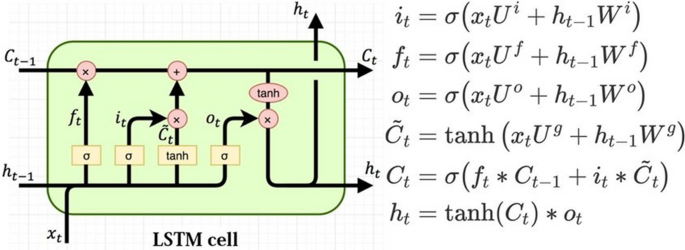
\includegraphics[width=0.6\linewidth]{chapters/neural/images/lstm.png}
	\caption{Схема LSTM}
	\label{img:lstm}
\end{figure}
Основная идея LSTM~\cite{hochreiter1997long} --- использование механизма \textbf{ячейки памяти} и набора \textbf{затворов (gates)}, которые регулируют, какая часть информации из предыдущих шагов будет запоминаться, забываться и выводиться на выход. Это позволяет LSTM ``удерживать'' важную информацию на более длинных промежутках.

\subsection{Структура LSTM-ячейки}
В классической LSTM-ячейке три затвора:
\begin{enumerate}
    \item \textbf{Forget gate} (затвор забывания) управляет тем, какая часть предыдущего состояния памяти $C_{t-1}$ будет \textit{забыта}.
    \item \textbf{Input gate} (затвор записи) определяет, какая часть нового кандидата состояния $\tilde{C}_t$ попадёт в текущее состояние памяти.
    \item \textbf{Output gate} (затвор выхода) определяет, какая часть текущего состояния памяти $C_t$ будет подана на выход $h_t$.
\end{enumerate}

Типичные формулы (безbias-термов):
\[
f_t = \sigma(W_f \cdot [h_{t-1}, x_t]), \quad
i_t = \sigma(W_i \cdot [h_{t-1}, x_t]), \quad
\tilde{C}_t = \tanh(W_C \cdot [h_{t-1}, x_t]),
\]
\[
C_t = f_t \odot C_{t-1} + i_t \odot \tilde{C}_t,
\]
\[
o_t = \sigma(W_o \cdot [h_{t-1}, x_t]), \quad
h_t = o_t \odot \tanh(C_t).
\]

\subsection{Продвинутые моменты LSTM}
\begin{itemize}
    \item \textbf{Bidirectional LSTM}: двунаправленная архитектура для учёта контекста слева и справа.
    \item \textbf{Stacked LSTM}: многослойные (глубокие) LSTM для повышения выразительности.
    \item \textbf{Dropout и Recurrent Dropout}: регуляризация занулением нейронов в связях.
    \item \textbf{Attention Mechanisms}: совмещение с механизмом внимания (Attention) для более гибкого «фокуса» на нужных шагах входной последовательности.
\end{itemize}

\subsection{Архитектура GRU}

\begin{figure}[h]
	\centering
	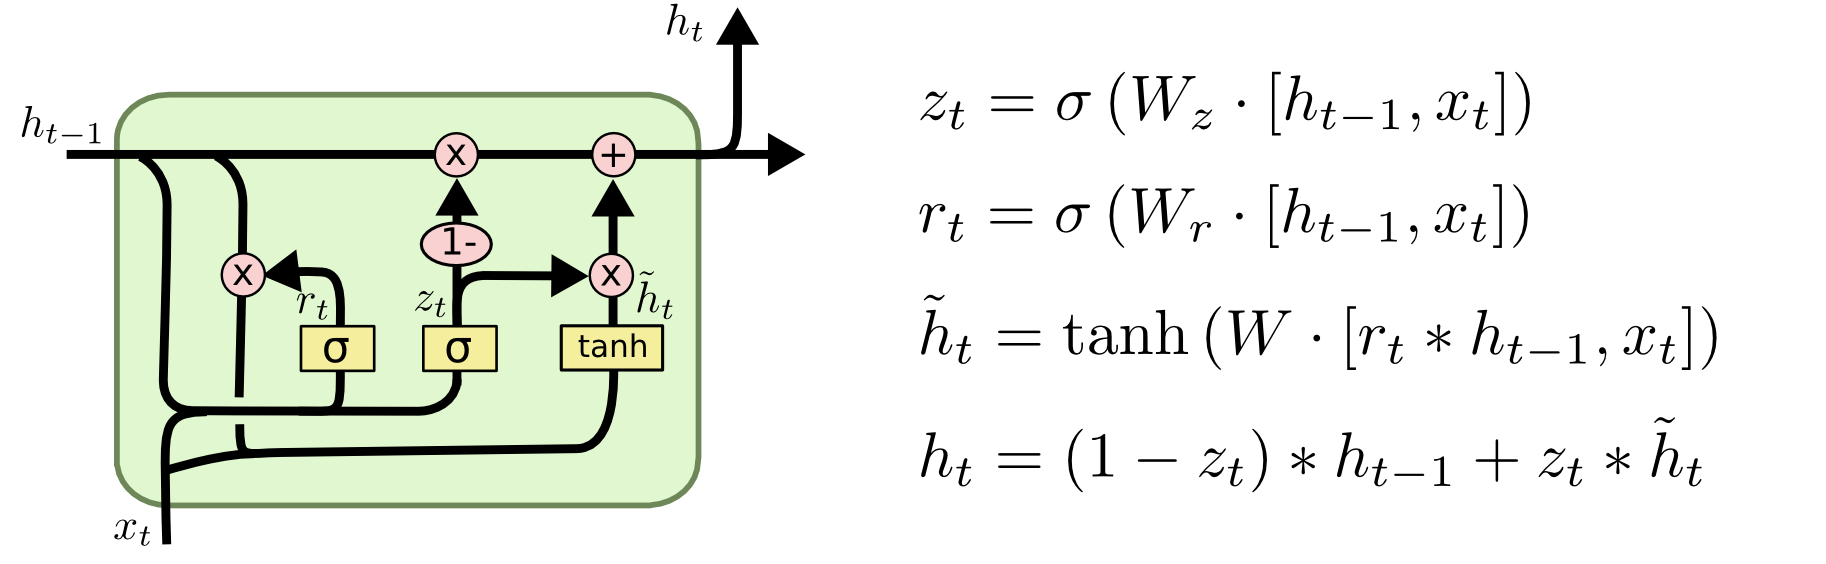
\includegraphics[width=0.6\linewidth]{chapters/neural/images/gru.png}
	\caption{Схема GRU}
	\label{img:gru}
\end{figure}
GRU (Gated Recurrent Unit) была предложена в работе~\cite{cho2014properties} как упрощение по сравнению с LSTM: используется всего два затвора (update и reset), что уменьшает число параметров модели.

\subsection{Структура GRU-ячейки}
\begin{enumerate}
    \item \textbf{Update gate} $z_t$ управляет тем, сколько информации из предыдущего выхода $h_{t-1}$ перенести в новое состояние.
    \item \textbf{Reset gate} $r_t$ определяет, сколько ``старой'' информации нужно сбросить перед вычислением текущего кандидата.
\end{enumerate}

Основные формулы:
\[
z_t = \sigma(W_z \cdot [h_{t-1}, x_t]), \quad
r_t = \sigma(W_r \cdot [h_{t-1}, x_t]),
\]
\[
\tilde{h}_t = \tanh \bigl(W_h \cdot [r_t \odot h_{t-1}, x_t]\bigr),
\]
\[
h_t = (1 - z_t)\odot h_{t-1} + z_t \odot \tilde{h}_t.
\]

\subsection{Преимущества GRU}
\begin{itemize}
    \item Меньше параметров по сравнению с LSTM, что может ускорять обучение.
    \item Часто качество на задачах NLP и временных рядах сопоставимо с LSTM.
\end{itemize}

\subsection{Продвинутые моменты GRU}
\begin{itemize}
    \item \textbf{Layer Normalization / BatchNorm}: нормализация на выходе или по слоям помогает стабилизировать обучение.
    \item \textbf{Residual/Skip Connections}: добавляются короткие связи для улучшения обратного распространения ошибки.
    \item \textbf{Bidirectional GRU}: аналогично двунаправленным LSTM, учитываем контекст с двух сторон.
\end{itemize}

\subsection{Сравнение LSTM и GRU}
\begin{itemize}
    \item LSTM имеет более гибкую структуру (три затвора, отдельное состояние $C_t$), но и больше параметров.
    \item GRU проще, часто обучается быстрее и даёт сравнимое качество.
\end{itemize}


\subsection{Теоретическая Задача 1: Анализ взрывающих и затухающих градиентов}
Объясните, почему в классической RNN (без затворов) возникает проблема затухающих и взрывающих градиентов при обучении на длинных последовательностях. Как архитектуры LSTM и GRU помогают смягчить эту проблему?

\begin{itemize}
    \item \textbf{Классическая RNN} использует повторяющиеся умножения весовых матриц на каждом временном шаге. Для длинных цепочек такие последовательные умножения могут привести к экспоненциальному затуханию или экспоненциальному росту (взрыв градиентов), поскольку собственные значения матриц многократно перемножаются.
    \item \textbf{LSTM и GRU} вводят механизмы затворов и явные пути прямой передачи градиента (``гейтированные'' или ``прямые'' связи через состояние), что существенно стабилизирует процесс обучения. Ячейка памяти LSTM (и аналогичная структура в GRU) создаёт путь, по которому градиент может проходить без постоянного перемножения на матрицу весов. Таким образом, модели меньше страдают от затухания или взрыва.
\end{itemize}

\subsection{Теоретическая Задача 2: Сравнение количества параметров в LSTM и GRU}
Предположим, что размерность входа равна $d$, а размер скрытого состояния равен $h$. Сравните (количественно) число обучаемых параметров в одной LSTM-ячейке и одной GRU-ячейке. Объясните, как это влияет на время обучения и возможность переобучения?

\begin{itemize}
    \item \textbf{LSTM} имеет 4 вычислительных ``ветви'' (forget, input, candidate, output), каждая включает матрицу весов для входа $W_{*}^{(x)}$ и для предыдущего скрытого состояния $W_{*}^{(h)}$, а также соответствующие bias. Итого для LSTM:
    \[
    \text{Параметры в LSTM} \approx 4 \cdot (d \cdot h + h \cdot h + h)
    \]
    \item \textbf{GRU} имеет 3 ветви (update, reset, candidate), что даёт формулу:
    \[
    \text{Параметры в GRU} \approx 3 \cdot (d \cdot h + h \cdot h + h)
    \]
    \item Таким образом, GRU имеет меньше параметров, что может приводить к более быстрой сходимости и меньшей склонности к переобучению (но и менее ``гибкой'' архитектуре в некоторых случаях).
\end{itemize}

\subsection{Теоретическая Задача 3: Пределы LSTM/GRU при очень длинных зависимостях}

Поясните, в каких случаях даже LSTM или GRU могут не справляться с очень длинными зависимостями? Предложите, какие механизмы или архитектуры способны улучшить качество работы с подобными зависимостями.

\begin{itemize}
    \item \textbf{Очень длинные зависимости}: даже с механизмами затворов для очень больших длин (например, сотни или тысячи временных шагов) LSTM/GRU могут всё ещё сталкиваться с трудностями в запоминании самых первых шагов. 
    \item \textbf{Mechanisms/архитектуры}: 
    \begin{itemize}
        \item \textbf{Attention} (применение в Encoder-Decoder архитектурах). Позволяет модели ``обращаться'' к нужным шагам напрямую, минуя долгую цепочку рекуррентных состояний.
        \item \textbf{Transformers}: полностью отказываются от рекуррентной структуры и используют механизм внимания (self-attention), что улучшает способность моделировать дальние зависимости.
        \item \textbf{Memory-augmented networks} (Neural Turing Machines, Memory Networks): явное внешнее хранилище.
    \end{itemize}
\end{itemize} 

\section{KAN как альтернативная базовая архитектура}
\subsection{Теорема Коллмогорова Арнольда}

В области машинного обучения многослойные персептроны (MLP) традиционно считаются универсальными аппроксиматорами функций. Однако существует менее известный, но не менее важный математический результат - теорема Колмогорова-Арнольда, которая предлагает альтернативный подход к представлению многомерных функций.
Теорема Колмогорова-Арнольда, доказанная в 1957 году, утверждает, что любая непрерывная функция нескольких переменных может быть представлена как суперпозиция непрерывных функций одной переменной и операции сложения. Формально это можно записать следующим образом:
\[
f(x_1, ..., x_n) = \sum_{q=1}^{2n+1} \Phi_q \left(\sum_{p=1}^n \phi_{q,p}(x_p)\right)
\]
где $\phi_{q,p}$ и $\Phi_q $ - непрерывные функции одной переменной.

Долгое время теорема Колмогорова-Арнольда считалась преимущественно теоретическим результатом без практического применения. Основная причина заключалась в том, что функции $\phi_{q,p}$ и $\Phi_q$ могут быть очень сложными и даже разрывными, что делает их непрактичными для численной реализации.

\subsubsection{Теоретическая задача 1: представление Колмогорова-Арнольда}
Приведите функцию $ f(x,y,z) = \frac{x^y}{z} $ в виде представления Колмогорова-Арнольда

\textbf{Решение:}
\[
f(x,y,z) = \frac{x^y}{z} = \exp(\exp(\log y + \log \log x) + (-\log z))
\]
\[
\Phi_1 = \exp
\]
\[
\phi_{1, 1} = \exp\log(y)
\]
\[
\phi_{1, 2} = \log\log(y)
\]
\[
\phi_{1, 3} = -\log z
\]

\subsection{Kolmogorov-Arnold Networks (KAN)}

Теорема Колмогорова-Арнольда вдохновила создание нового класса нейронных сетей - сетей Колмогорова-Арнольда (KAN), которые предлагают альтернативу традиционным многослойным персептронам. В то время как MLP используют фиксированные функции активации на узлах ("нейронах"), KAN размещает обучаемые функции активации на рёбрах ("весах") и реализует их с помощью B-сплайнов.
B-сплайны представляют собой кусочно-полиномиальные функции, обладающие рядом важных свойств:
\begin{itemize}
    \item Локальность: изменение одного контрольного узла влияет только на ограниченную область функции
    \item Гладкость: B-сплайны обеспечивают заданную степень непрерывности производных
    \item Компактность: эффективное представление сложных функций с небольшим числом параметров
\end{itemize}

Формально, слой KAN с входной размерностью $n_{in}$ и выходной размерностью $n_{out}$ можно определить как матрицу одномерных функций:
\[
\Phi(X) = {\phi_{q,p}}, p = 1,2,\ldots,n_{in}, q = 1,2,\ldots,n_{out}
\]
где каждая функция $\phi_{q,p}$ параметризована как B-сплайн с обучаемыми коэффициентами.

Главным отличием от исходной теоремы в KAN является уход от фиксированной глубины. Полная нейронная сеть представляет из себя композицию слоёв, то есть последовательное применение функциональных матриц:
\[
KAN(X) = \Phi_n(\Phi_{n - 1}( ...\Phi_2(\Phi_1(X))...))
\]

Исследования показывают, что KAN могут достигать сравнимой или лучшей точности по сравнению с более крупными MLP при использовании значительно меньшего количества параметров. Например, для решения дифференциальных уравнений в частных производных двухслойная KAN шириной 10 может быть в 100 раз точнее и в 100 раз эффективнее по параметрам, чем четырехслойная MLP шириной 100.

\subsubsection{Теоретическая задача 2: сети Колмогорова-Арнольда}
Покажите, как использовать обратное распространениие ошибки для обучения KAN.

\textbf{Решение:}

Использование B-сплайна в определении слоя затрудняет прямое применение обратного распространения ошибки, так как его производная в каждой точке заранее неизвестна. Однако каждый B-сплайн можно заменить на скрытый слой из перцептронов с одним входом и разными функциями активации, соответствующими базисным функциям сплайна, производные которых известны заранее. Таким образом KAN сводится к традиционной нейронной сети.

\subsection{КАН для обучения без учителя}

Сети Колмогорова-Арнольда могут быть эффективно адаптированы для задач обучения без учителя, что открывает новые возможности для анализа данных и научных открытий. В отличие от традиционного применения в задачах обучения с учителем, KAN для обучения без учителя фокусируются на поиске скрытых зависимостей в данных без явного указания целевых переменных.
Основная идея заключается в преобразовании задачи обучения без учителя в специальную форму обучения с учителем. Пусть имеется набор признаков $(x_1, x_2, ..., x_d)$, среди которых предполагается наличие функциональных зависимостей. Цель состоит в поиске нетривиальной функции $f$, такой что:
\[
f(x_1, x_2, ..., x_d) \approx 0
\]

Для решения этой задачи используется контрастивный подход, где определяются:
Позитивные примеры: реальные наборы признаков
Негативные примеры: наборы признаков с случайной перестановкой значений

KAN обучается различать эти два класса примеров, используя специальную модификацию архитектуры с гауссовой функцией активации в последнем слое:
\[
KAN_{unsupervised}(X) = \delta (KAN(X)), \text{ где } \delta(x) = \exp(-\frac{x^2}{2w^2})
\]
Такой подход позволяет KAN автоматически обнаруживать нетривиальные зависимости в данных. Например, в физических экспериментах сеть может выявлять фундаментальные законы природы, анализируя только измеренные величины.

\subsubsection{Теоретическая задача 3: KAN без учителя}
Какой датасет и какая архитектура KAN нужна для переоткрытия второго закона Ньютона?

\textbf{Решение:}

Набор данных должен содержать следующие измерения:
\begin{itemize}
    \item массы тел (m)
    \item приложенных сил (F)
    \item наблюдаемых ускорений (a)
\end{itemize}

Выражение меняется на:
\[
F=ma\rightarrow F-ma=0
\]
Далее представим это выражение в виде KAN:
\[
KAN(F, m, a) = \delta\left( F-\exp\left( \log m + \log a \right) \right),
\]
\[
\text{ где } \exp, \log \text{ - B-сплайны, определяемые во время обучения}
\]
Для обучения настоящие данные будут иметь целевую переменную равную 1, а случайно созданные - 0. Полученные в результате обучения функции позволят получить правильный вид закона.



\begin{thebibliography}{99}
\bibitem{hochreiter1997long} S.~Hochreiter, J.~Schmidhuber, \textit{Long short-term memory.} Neural Computation, 9(8), 1735--1780, 1997.
\bibitem{cho2014properties} K.~Cho, B.~van Merrienboer, D.~Bahdanau, Y.~Bengio, \textit{On the properties of neural machine translation: Encoder-decoder approaches.} arXiv preprint arXiv:1409.1259, 2014.
\end{thebibliography}

\section*{Быстрые методы стохастического градиента: Поляка и Нестерова}

Методы ускорения градиентного спуска применяются для уменьшения количества итераций, необходимых для достижения минимума функции потерь. Два важных метода для ускорения сходимости — это метод накопления инерции (Momentum) Поляка и метод ускоренного градиента Нестерова.


\subsection*{Метод Поляка (Momentum)}

Метод Поляка использует понятие \textit{накопленной скорости} для сглаживания обновления параметров и уменьшения колебаний. Вместо прямого шага в направлении градиента, метод учитывает предыдущие обновления. Формулы метода:

\begin{equation*}
\begin{aligned}
    v &:= \gamma v + (1 - \gamma) \nabla \mathcal{L}(w, x_i), \\
    w &:= w - \eta v,
\end{aligned}
\end{equation*}
где $\gamma \in [0, 1)$ — коэффициент импульса, $\eta$ — шаг обучения, $\nabla \mathcal{L}(w, x_i)$ — градиент функции потерь для $x_i$, $v$ — накопленная скорость.

Таким образом, метод Поляка комбинирует текущий градиент с предыдущими направлениями движения, что позволяет "разгоняться" в одном направлении и сглаживать траекторию на плоских участках.

\subsection*{Метод Нестерова (Nesterov Accelerated Gradient, NAG)}

Метод Нестерова представляет собой модификацию метода Поляка, где используется идея предварительного "предсказания" положения параметров. Основное отличие в том, что градиент рассчитывается не в текущей точке, а в точке, смещённой в направлении скорости. Формулы обновления параметров:
\begin{equation*}
\begin{aligned}
    v &:= \gamma v + (1 - \gamma) \nabla \mathcal{L}(w - \eta \gamma v, x_i), \\
    w &:= w - \eta v.
\end{aligned}
\end{equation*}

"Заглядывание вперёд" в направлении текущей скорости позволяет более точно учитывать геометрию функции и улучшать сходимость. Это позволяет методу Нестерова минимизировать колебания и снижать избыточные шаги в направлении градиента.

\subsection*{Графическое объяснение методов}

\begin{figure}[h!]
    \centering
    \begin{minipage}[t]{0.45\textwidth}
        \centering
        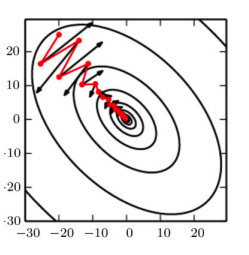
\includegraphics[width=0.9\textwidth]{chapters/neural/images/polyak.png}
        \\[0.5em]
        Рис. 1: Метод Поляка (Momentum)
    \end{minipage}%
    \hfill
    \begin{minipage}[t]{0.45\textwidth}
        \centering
        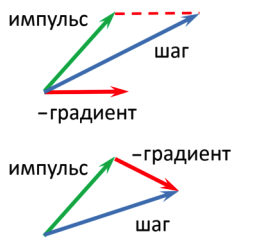
\includegraphics[width=0.9\textwidth]{chapters/neural/images/nesterov.png}
        \\[0.5em]
        Рис. 2: Метод Нестерова (NAG)
    \end{minipage}
\end{figure}

\begin{itemize}
    \item На левом рисунке показано, как метод Поляка сглаживает путь оптимизации за счёт накопленного импульса.
    \item На правом рисунке метод Нестерова использует "предсказание" положения параметров, что приводит к более оптимальному шагу.
\end{itemize}

\subsection*{Сравнение методов}
    \item - Метод Поляка прост в реализации и хорошо работает на негладких функциях.

    \item - Метод Нестерова обеспечивает более высокую скорость сходимости благодаря использованию информации о кривизне.

    \item - Оба метода легко интегрируются в современные алгоритмы оптимизации, такие как Adam и RMSProp.

\subsection*{Задача 1}
Рассмотрим функцию
\[
f(w) = w^2.
\]
Примените метод градиентного спуска с импульсом Поляка для минимизации этой функции. Шаг обучения $\eta = 0.1$, коэффициент импульса $\gamma = 0.9$, начальная точка $w_0 = 5$. Выполните три итерации.

\textbf{Решение:}

\[
v_t = \gamma v_{t-1} + (1 - \gamma) \nabla f(w_t), \quad w_{t+1} = w_t - \eta v_t,
\]
где $v_t$ — накопленная скорость, $\nabla f(w_t)$ — градиент функции $f(w) = w^2$, а $\eta$ — шаг обучения.

1.
   \[
   w_0 = 5, \quad v_0 = 0, \quad \nabla f(w_0) = 2w_0 = 10.
   \]
   \[
   v_1 = 0.9 \cdot 0 + (1 - 0.9) \cdot 10 = 1, \quad w_1 = 5 - 0.1 \cdot 1 = 4.9.
   \]

2.
   \[
   w_1 = 4.9, \quad \nabla f(w_1) = 9.8.
   \]
   \[
   v_2 = 0.9 \cdot 1 + (1 - 0.9) \cdot 9.8 = 1.88, \quad w_2 = 4.9 - 0.1 \cdot 1.88 = 4.712.
   \]

3.
   \[
   w_2 = 4.712, \quad \nabla f(w_2) = 9.424.
   \]
   \[
   v_3 = 0.9 \cdot 1.88 + (1 - 0.9) \cdot 9.424 = 2.634, \quad w_3 = 4.712 - 0.1 \cdot 2.634 = 4.448.
   \]

\textbf{Ответ:} после трёх итераций метода Поляка значение параметра $w$ уменьшилось с 5 до $4.448$ - он движется в сторону минимума функции $f(w) = w^2$.

\subsection*{Задача 2}
Для функции 
\begin{equation*}
    f(w) = (w - 3)^2 + 7
\end{equation*}
выполните две итерации метода Нестерова с параметрами $\eta = 0.2$ и $\gamma = 0.8$, начиная с $w = -1$. Найдите значения $w$ после каждой итерации.

\textbf{Решение:}
\begin{equation*}
    v_k = \gamma v_{k-1} + (1 - \gamma) \nabla f(w_k - \eta \gamma v_{k-1}), \quad w_{k+1} = w_k - \eta v_k.
\end{equation*}
1.
\[
   w_0 = -1, \quad v_0 = 0, \quad \nabla f(-1) = 2(-1 - 3) = -8.
\]
\[ v_1 = 0.8 \cdot 0 + 0.2 \cdot (-8) = -1.6, \quad w_1 = -1 - 0.2 \cdot (-1.6) = -0.68. \]
2. 
\[
   w_1 = -0.68, \quad v_1 = -1.6, \quad \nabla f(-0.68 - 0.2 \cdot 0.8 \cdot (-1.6)) = -6.848.
\]
\[ v_2 = 0.8 \cdot (-1.6) + 0.2 \cdot (-6.848) = -2.08, \quad w_2 = -0.68 - 0.2 \cdot (-2.08) = -0.272. \]

\textbf{Ответ:} после двух итераций значение $w$ изменилось с $-1$ до $-0.272$.

\subsection*{Задача 3}
Рассмотрим функцию:  
 \item\( f_1(w) = 10w_1^2 + w_2^2 \) (вытянутая квадратичная функция)   

Предположим, что для минимизации используется либо метод Поляка (Momentum), либо метод Нестерова (NAG).  
\item Начальная точка: \( w_0 = (10, 5) \),  шаг обучения \( \eta = 0.1 \),   коэффициент импульса \( \gamma = 0.9 \).  

Укажите, какой метод будет эффективнее и почему.

\textbf{Решение:}

1. Градиенты в направлении \( w_1 \) (\( \nabla_{w_1} f = 20w_1 \)) гораздо больше, чем в направлении \( w_2 \) (\( \nabla_{w_2} f = 2w_2 \)). Это приводит к "зигзагообразным" траекториям.

2. Начальная точка \( w_0 = (10, 5) \) находится далеко от минимума (\( w^* = (0, 0) \)). Ошибки по каждой координате значительно различаются, что увеличивает влияние масштабирования на скорость сходимости.

Метод Поляка не учитывает \textit{предсказание будущего положения}, поэтому траектория часто оказывается менее оптимальной в условиях вытянутости. Это может привести к увеличению числа итераций.

Метод Нестерова строит обновление на основе "предсказанной" точки \( w_t - \eta \gamma v_t \), заглядывая вперёд в направлении текущей скорости \( v_t \). Для вытянутых функций это даёт два преимущества:

1. Лучшее согласование шага с направлением градиента:  
    метод Нестерова корректирует траекторию, уменьшает зигзагообразность и быстрее приближается к минимуму.

2. Ускорение сходимости по оси с меньшим масштабом:  
   "заглядывание" даёт возможность быстрее компенсировать медленное движение вдоль более плоской оси \( w_2 \).

\textbf{Вывод: } для данной функции \( f_1(w) = 10w_1^2 + w_2^2 \) метод Нестерова (NAG) будет эффективнее, чем метод Поляка (Momentum), который хотя и полезен для сглаживания колебаний, менее адаптивен к вытянутой геометрии задачи, что приводит к более медленной сходимости.
